
\section{Chemical equilibrium from a thermodynamic and mathematical perspective}

% --------------------------------------------------------------------------------------------------------------------%
% Chemical equilibrium from a thermodynamic perspective
% --------------------------------------------------------------------------------------------------------------------%
\subsection{Gibbs energy minimization and its constraints}
%
\begin{frame}{Chemical equilibrium from a thermodynamic perspective}
\begin{itemize}
\item A system under prescribed temperature $T$ and pressure $P$ is in
chemical equilibrium if its \textbf{Gibbs energy} $G$ is at a minimum. 
\begin{itemize}
\item this results from the \emph{second law of thermodynamic} that says
that a system tends to a state of maximum entropy $S$. 
\item the minimum Gibbs energy condition arises because $G := H - T\,S$, where
$H$ is enthalpy. 
\item \textbf{Note}: \\
\alert{\textbf{Entropy}} $S$ is the measure of a system's thermal energy per unit temperature that is unavailable for doing useful work. \\ 
\alert{\textbf{Enthalpy}} $H$ is a property of a thermodynamic system, defined as the sum of the system's internal energy and the product of its pressure and volume.
\end{itemize}
\pause
\item Analogy to the \textbf{mechanical equilibrium}: a \emph{ball rolling down a hill}. 
We want to find the \textbf{final position} of the ball that results in a minimum for its 
\textbf{potential energy}.
\pause
\item In thermodynamics, we want to find the \textbf{composition (amounts of each species)}, in every phase, that \textbf{minimizes the Gibbs energy} of the chemical system.
\end{itemize}
\end{frame}
%
% --------------------------------------------------------------------------------------------------------------------%
% Constraints in a chemical equilibrium state
% --------------------------------------------------------------------------------------------------------------------%
%
\begin{frame}{Constraints in a chemical equilibrium state}
\begin{itemize}
\item In \alert{\textbf{mechanical equilibrium}}, a ball rolling down a hill is \textbf{constrained by its surface topology}. 
\pause
\item In \textbf{thermodynamics}, the species in a chemical system seeking a state of chemical
equilibrium is also \textbf{constrained by some conditions}: 
\begin{itemize}
\item \textbf{its nonnegativity} (species amounts cannot be negative),
\item \alert{\textbf{mass conservation}}.
\end{itemize}
\end{itemize}
\end{frame}
%
%
% --------------------------------------------------------------------------------------------------------------------%
% Mass conservation constraints in chemical equilibrium
% --------------------------------------------------------------------------------------------------------------------%
%
\begin{frame}{Mass conservation constraints in chemical equilibrium \, i}
%
\vskip 10pt
To illustrate \alert{\textbf{mass conservation constraints}} the following problem: 
\begin{itemize}
\item mix 100 moles of H$_{2}$O and 2 moles of CO$_{2}$
and \textbf{calculate the equilibrium state of the system}. 
\item these two substances will react and form several species (H$^{+}$,
HCO$_{3}^{-}$ etc.).
\end{itemize}
\hiddenpause
\alert{\textbf{Quiz}}: at chemical equilibrium, what can we tell about 
the amounts of H, O, C, Z?

\begin{center}
\href{http://etc.ch/oyhr}{\textcolor{indigo(dye)}{\tt http://etc.ch/oyhr}} 
\quad
or 
\quad

\includegraphics[height=0.21\columnwidth]{figures/chemical-equilibrium/poll-mass-balance.png}
\end{center}

\hiddenpause
\textbf{Answer}: 200 mols of H, 104 mols of O, and 2 mols of C,  the final charge must be equal to the initial charge. 
\end{frame}
%
\begin{frame}{Mass conservation constraints in chemical equilibrium\, ii}
	%
\begin{itemize}
		\item Calculating chemical equilibrium requires finding a composition for
		the system (i.e., amount of species, usually defined by vector 
		$n = [n_{\sf H^{+}}, n_{\sf HCO_{3}^{-}}, \ldots]$) that 
		\textbf{minimizes its Gibbs energy} and simultaneously satisfies 
		\alert{\textbf{mass conservation}} of:
		\begin{itemize}
			\item \textbf{chemical elements}; and
			\item \textbf{electric charge}.
		\end{itemize}
		\pause
		\item \alert{\textbf{Note}}: we use the term \alert{\textbf{elements}} represented by vector $b$ 
		to denote both \emph{chemical elements} and \emph{electric charge}, i.e., 
		$b = [b_{\sf H}, b_{\sf O}, b_{\sf C}, b_{\sf Z}]$.
	\end{itemize}
\end{frame}
%
% --------------------------------------------------------------------------------------------------------------------%
% Chemical equilibrium problem for the H2O–CO2 system
% --------------------------------------------------------------------------------------------------------------------%
%
\begin{frame}{Chemical equilibrium problem for the H$_{\boldsymbol{2}}$O–CO$_{\boldsymbol{2}}$
system}

\lcol

Given \emph{temperature} $T$, \emph{pressure} $P$ and the \emph{amounts
of elements} H, O, C, determine \\
the \textbf{amounts of the species at equilibrium}:
\begin{center}
\begin{tabular}{cc}
\toprule 
\multicolumn{1}{c}{\textbf{Aqueous Phase}} & \multicolumn{1}{c}{\textbf{Gaseous Phase}}\tabularnewline
\midrule
H$_{2}$O(aq) & CO$_{2}$(g)\tabularnewline
H$^{+}$(aq) & H$_{2}$O(g)\tabularnewline
OH$^{-}$(aq) & \tabularnewline
CO$_{3}^{2-}$(aq) & \tabularnewline
HCO$_{3}^{-}$(aq) & \tabularnewline
CO$_{2}$(aq) & \tabularnewline
\bottomrule
\end{tabular} 
\par\end{center}

\rcol
\pause
\vskip 5pt
\alert{\textbf{Questions:}}
\begin{itemize}
\item What are the amounts of each chemical species at equilibrium? 
\item Which phases exist at equilibrium? 
\item How much carbon dioxide, CO$_{2}$(g), dissolved as carbon-bearing
aqueous species? 
\item How much solvent water, H$_{2}$O(aq), evaporated to the gas phase
as vapor H$_{2}$O(g)? 
\item What is the concentration of H$^{+}$(aq), which is related to pH
(acidity)?
\end{itemize}
\ecol
\end{frame}
%
% --------------------------------------------------------------------------------------------------------------------%
% Mass conservation constraints for the H2O–CO2 system at equilibrium
% --------------------------------------------------------------------------------------------------------------------%
%
\begin{frame}[<+->]{Mass conservation constraints for the H$_{\boldsymbol{2}}$O–CO$_{\boldsymbol{2}}$
system at equilibrium}
 
\begin{itemize}
\item At equilibrium, the amounts of the species:
\[
n=(n_{\mathsf{H_{2}O\text{(aq)}}},\;n_{\mathsf{H^{+}\text{(aq)}}},\;n_{\mathsf{OH^{-}\text{(aq)}}},\;n_{\mathsf{CO_{3}^{2-}\text{(aq)}}},\;n_{\mathsf{HCO_{3}^{-}}\text{(aq)}},\;n_{\mathsf{CO_{2}\text{(aq)}}},\;n_{\mathsf{CO_{2}\text{(g)}}},\;n_{\mathsf{H_{2}O\text{(g)}}})
\]
must satisfy the \textbf{mass conservation equations} for each element:{\small{}
\begin{alignat}{1}
2n_{\mathsf{H_{2}O\text{(aq)}}}+n_{\mathsf{H^{+}\text{(aq)}}}+n_{\mathsf{OH^{-}\text{(aq)}}}+n_{\mathsf{HCO_{3}^{-}\text{(aq)}}}+2n_{\mathsf{H_{2}O\text{(g)}}} & =b_{\mathsf{H}}\\
n_{\mathsf{H_{2}O\text{(aq)}}}+n_{\mathsf{OH^{-}\text{(aq)}}}+3n_{\mathsf{CO_{3}^{2-}\text{(aq)}}}+3n_{\mathsf{HCO_{3}^{-}}\text{(aq)}}+2n_{\mathsf{CO_{2}\text{(aq)}}}+2n_{\mathsf{CO_{2}\text{(g)}}}+n_{\mathsf{H_{2}O\text{(g)}}} & =b_{\mathsf{O}}\\
n_{\mathsf{CO_{3}^{2-}\text{(aq)}}}+n_{\mathsf{HCO_{3}^{-}\text{(aq)}}}+n_{\mathsf{CO_{2}\text{(aq)}}}+n_{\mathsf{CO_{2}\text{(g)}}} & =b_{\mathsf{C}}\\
n_{\mathsf{H^{+}\text{(aq)}}}-n_{\mathsf{OH^{-}\text{(aq)}}}-2n_{\mathsf{CO_{3}^{2-}\text{(aq)}}}-n_{\mathsf{HCO_{3}^{-}\text{(aq)}}} & =b_{\mathsf{Z}}
\end{alignat}
}{\small\par}
\item \alert{\textbf{Exercise}}: Show that, for this specific system, the conservation
equation for electrical charge, Z, is \emph{linearly dependent} on
the other equations.
%\item \alert{\textbf{Hint}}: Show that the last row 
%(4) = (1) - 2 (2) + 4 (3).

\end{itemize}
\end{frame} 
%
% --------------------------------------------------------------------------------------------------------------------%
% Mass conservation constraints written in matrix form
% --------------------------------------------------------------------------------------------------------------------%
%
\begin{frame}{Mass conservation constraints written in matrix form}

The mass balance equations can be written in matrix form: \\[10pt]

\begin{cbox}{Mass conservation equation in matrix form}{\Large{}
\[
An=b
\]
}\end{cbox}where:
\begin{itemize}
\item $A$ is the \textbf{formula matrix} of the system
\item $n=(n_{1},\ldots,n_{\text{N}})$ is the \textbf{vector of species
amounts}
\item $b=(b_{1},\ldots,b_{\text{E}})$ is the \textbf{vector of element
amounts}
\end{itemize}
\end{frame}
%
% --------------------------------------------------------------------------------------------------------------------%
% Constructing the formula matrix for the H2O–CO2 system
% --------------------------------------------------------------------------------------------------------------------%
%
\begin{frame}[<+->]{Constructing the formula matrix for the H$_{\boldsymbol{2}}$O–CO$_{\boldsymbol{2}}$ system\; i}

Consider the following ordering for species and elements in the system:
\begin{center}
\begin{tabular*}{1\textwidth}{@{\extracolsep{\fill}}ccccc}
\toprule 
\textbf{Index} & \textbf{Species} &  & \textbf{Index} & \textbf{Element}\tabularnewline
\midrule
0 & H$_{2}$O(aq) &  & 0 & H\tabularnewline
1 & H$^{+}$(aq) &  & 1 & O\tabularnewline
2 & OH$^{-}$(aq) &  & 2 & C\tabularnewline
3 & CO$_{3}^{2-}$(aq) &  & 3 & Z\tabularnewline
4 & HCO$_{3}^{-}$(aq) &  &  & \tabularnewline
5 & CO$_{2}$(aq) &  &  & \tabularnewline
6 & CO$_{2}$(g) &  &  & \tabularnewline
7 & H$_{2}$O(g) &  &  & \tabularnewline
\bottomrule
\end{tabular*}
\par\end{center}

\alert{\textbf{Exercise:}} Construct the formula matrix $A$ for this system, where \\
\alert{\textbf{the coefficient $A_{ij}$ characterises the contribution of species 
$i$ into the element $j$}}. 
\end{frame}
%
% --------------------------------------------------------------------------------------------------------------------%
% Constructing the formula matrix for the H2O–CO2 system
% --------------------------------------------------------------------------------------------------------------------%
%
\begin{frame}{Constructing the formula matrix for the H$_{\boldsymbol{2}}$O-CO$_{\boldsymbol{2}}$ system\; ii}

\textbf{Answer:} {\small
$$A=\kbordermatrix{
& \mathclap{\mathsf{H_2O(aq)}} & \mathclap{\mathsf{H^+(aq)}} & \mathclap{\mathsf{OH^-(aq)}} & \mathclap{\mathsf{CO_3^{2-}(aq)}} & \mathclap{\mathsf{HCO_3^-(aq)}} & \mathclap{\mathsf{CO_2(aq)}} & \mathclap{\mathsf{CO_2(g)}}  & \mathclap{\mathsf{H_2O(g)}}\\
\mathsf{H} & \w{2} & \w{1} & \w{1} & \w{0} & \w{1} & \w{0} & \w{0} & \w{2}\\
\mathsf{O} & 1 & 0 & 1 & 3 & 3 & 2 & 2 & 1\\
\mathsf{C} & 0 & 0 & 0 & 1 & 1 & 1 & 1 & 0\\
\mathsf{Z} & 0 & 1 & \minus{1} & \minus{2} & \minus{1} & 0 & 0 & 0
}
$$}

\hiddenpause

\lcol

\alert{\textbf{Quiz:}} Which of the following linearly dependency relation
is true for the rows of $A$:

\vskip 5pt
\visible<2->{
\centering
\href{http://etc.ch/UbWW}{\textcolor{indigo(dye)}{\tt  http://etc.ch/oyhr}} \quad or \quad 

\includegraphics[height=0.35\columnwidth]{figures/chemical-equilibrium/poll-linear-independence.png}}

\rcol

\vspace{-4ex}
\visible<2->{
{\small{}
\begin{alignat*}{2}
\text{(1)} & \quad & \text{row(Z)} & =\text{row(H)}-2\,\text{row(O)}\\
\text{(2)} &  & \text{row(Z)} & =\text{row(H)}-2\,\text{row(O)}+2\,\text{row(C)}\\
\text{(3)} &  & \text{row(Z)} & =\text{row(H)}-2\,\text{row(O)}+4\,\text{row(C)}\\
\text{(4)} &  & \text{row(Z)} & =\text{row(H)}-2\,\text{row(O)}+6\,\text{row(C)}
\end{alignat*}
}{\small\par}
}
\visible<3->{
\textbf{Answer:} (3)
}
\ecol
\end{frame}
%
% --------------------------------------------------------------------------------------------------------------------%
% Calculating the amounts of elements from species amounts
% --------------------------------------------------------------------------------------------------------------------%
%
\begin{frame}{Calculating the amounts of elements from species amounts}

\vskip 10pt
\lcol[0.7]

\alert{\textbf{Exercise:}} Given 
\[
n=\left[\begin{array}{l}
n_{\mathsf{H_{2}O\text{(}aq\text{)}}}\\
n_{\mathsf{H^{+}\text{(}aq\text{)}}}\\
n_{\mathsf{OH^{-}\text{(}aq\text{)}}}\\
n_{\mathsf{CO_{3}^{2-}\text{(}aq\text{)}}}\\
n_{\mathsf{HCO_{3}^{-}\text{(}aq\text{)}}}\\
n_{\mathsf{CO_{2}\text{(}aq\text{)}}}\\
n_{\mathsf{CO_{2}\text{(}g\text{)}}}\\
n_{\mathsf{H_{2}O\text{(}g\text{)}}}
\end{array}\right]=\begin{bmatrix}n_{0}\\
n_{1}\\
n_{2}\\
n_{3}\\
n_{4}\\
n_{5}\\
n_{6}\\
n_{7}
\end{bmatrix}=\begin{bmatrix}55.4551\\
1.23485\cdot10^{-4}\\
8.39739\cdot10^{-11}\\
4.93648\cdot10^{-11}\\
1.23484\cdot10^{-4}\\
0.032861\\
1.96702\\
0.0531732
\end{bmatrix},
\]

\rcol[0.3]
calculate
\[
b=\left[\begin{array}{l}
b_{\mathsf{H}}\\
b_{\mathsf{O}}\\
b_{\mathsf{C}}\\
b_{\mathsf{Z}}
\end{array}\right] = A \, n.
\]
\ecol
\vskip 10pt
%\visible<2->{If we have vector $n$ and matrix $A$ we can compute $b = A n$.} \\
\visible<2->{Instead of doing such calculation manually (tedious and error prone), let's use \textbf{Python}: 
\begin{itemize}
\item for Python shell, you can use an online tool \href{http://repl.it/languages/python}{\textcolor{indigo(dye)}{\tt repl.it/languages/python}}
\item Python source code can be downloaded from \href{https://polybox.ethz.ch/index.php/s/ku86DyuR6nvW2Zl}{\textcolor{indigo(dye)}{\it mass-balance-with-blanks.py}}.
\end{itemize}
}
\end{frame}
%
% --------------------------------------------------------------------------------------------------------------------%
% Calculating the amounts of elements using Python
% --------------------------------------------------------------------------------------------------------------------%
%
\begin{frame}[fragile, allowframebreaks]{Calculating the amounts of elements using Python -- Source}

\lstinputlisting[language=Python, caption=Calculating the amounts of elements using Python]{python-files/mass-balance-with-blanks.py}	

\end{frame}
%
% --------------------------------------------------------------------------------------------------------------------%
% Calculating the amounts of elements using Python – Output
% --------------------------------------------------------------------------------------------------------------------%
%
\begin{frame}[fragile]{Calculating the amounts of elements using Python -- Output}

The Python code has to have the following output:

\begin{lstlisting}[language=Python, caption=Calculating the amounts of elements using Python -- Output]
Element H has 111.0168 moles and 111.8938 grams
Element O has 59.5084 moles and 952.0988 grams
Element C has 2.0000 moles and 24.0215 grams
Element Z has 0.0000 moles and 0.0000 grams

Species H2O(aq) has 5.5455e+01 moles and 9.9903e+02 grams
Species H+ has 1.2349e-04 moles and 1.2446e-04 grams
Species OH- has 8.3974e-11 moles and 1.4282e-09 grams
Species CO3-- has 4.9365e-11 moles and 2.9623e-09 grams
Species HCO3- has 1.2348e-04 moles and 7.5346e-03 grams
Species CO2(aq) has 3.2861e-02 moles and 1.4462e+00 grams
Species CO2(g) has 1.9670e+00 moles and 8.6568e+01 grams
Species H2O(g) has 5.3173e-02 moles and 9.5793e-01 grams
\end{lstlisting}

\textbf{Answer}: To check the correctness of the gaps in the code, use the  \href{https://polybox.ethz.ch/index.php/s/sVotdOJMkp740Lw}{\textcolor{indigo(dye)}{\it source code}}.

\end{frame}
%
% --------------------------------------------------------------------------------------------------------------------%
% Chemical equilibrium formulated as Gibbs energy minimization problem
% --------------------------------------------------------------------------------------------------------------------%
%
\begin{frame}{Chemical equilibrium formulated as Gibbs energy minimization problem}
%
\begin{cbox}{Gibbs energy minimization (GEM) problem}

Given temperature $T$, pressure $P$, and amounts of elements ${b=(b_{1},\ldots,b_{\text{E}})}$,
find the amounts of species ${n=(n_{1},\ldots,n_{\text{N}})}$ that
solve the \textbf{constrained minimization problem}:
\[
\min_{n}G(n;T,P)\qquad\text{subject to}\qquad An=b\quad\text{and}\quad n\geq0.
\]

\end{cbox}where:

\begin{itemize}
\item $G$ is the Gibbs energy of the system, a function of $n=(n_{1},\ldots,n_{\text{N}})$
as well as temperature $T$ and pressure $P$;
\item $An=b$ are the mass conservation constraints for each element;
\item $n\geq0$ are the non-negative constraints for the amounts of each
species.
\end{itemize}
\end{frame}
%
\begin{frame}{Gibbs energy function}

\begin{itemize}
\item 
\textbf{The Gibbs energy function}, $G$, is defined as: 
\[
\boxed{
G=\sum_{i=1}^{\text{N}}n_{i}\mu_{i},
}
\]
where $\mu_{i}$ is the \alert{\bf chemical potential} of the $i$th
species. \\[30pt]
%\hiddenpause
%\item \textbf{Question:} What is the dimension (in SI units) of $G$ and
%$\mu_{i}$? 
%\hiddenpause
\item $G$ has units of J, and $\mu_{i}$ units of J/mol.
\end{itemize}
\end{frame}
%
% --------------------------------------------------------------------------------------------------------------------%
% Chemical potential and its interpretation
% --------------------------------------------------------------------------------------------------------------------%
%
\subsection{Chemical potential of chemical species}
%
\begin{frame}{Chemical potential and its interpretation}

\begin{itemize}
\item The \textbf{chemical potential of a substance $\mu_{i}$} is a measure of
its tendency to transform into other substances.
\pause
\item In the following reaction:
\[
\mathsf{A\rightleftharpoons B},
\]

\begin{itemize}
\item $\mu_{\sf A}>\mu_{\sf B}$: substance A will tend to transform to B 
\item $\mu_{\sf A}=\mu_{\sf B}$: substances A and B are in equilibrium, no
transformation is happening
\item $\mu_{\sf A}<\mu_{\sf B}$: substance B will tend to transform to A
\end{itemize}
\pause
\item The higher the value of $\mu_{\sf A}$, the higher the tendency for A
to transform to B.
\end{itemize}
\end{frame}
%
% --------------------------------------------------------------------------------------------------------------------%
% Chemical potential and its interpretation – Example
% --------------------------------------------------------------------------------------------------------------------%
%
\begin{frame}{Chemical potential and its interpretation, Example}
\begin{itemize}
\item Consider the following reaction:
\[
\mathsf{CO_{2}\text{(g)}\rightleftharpoons CO_{2}\text{(aq)}}
\]
\vskip -50pt

\includegraphics[height=0.17\columnwidth,right]{figures/chemical-equilibrium/poll-linear-independence.png}
\pause
\vskip -40pt
\item We have the following three cases: 
{
\footnotesize{}
\begin{align*}
\text{\textbf{Case I}} &  & \textbf{Case II} &  & \textbf{Case III}\\
\mu_{\mathsf{CO_{2}\text{(g)}}} & = -390.347\,{\mathsf{kJ/mol}} & 
\mu_{\mathsf{CO_{2}\text{(g)}}} & = -390.347\,{\mathsf{kJ/mol}} & 
\mu_{\mathsf{CO_{2}\text{(g)}}} & = -389.185\,{\mathsf{kJ/mol}}\\
\mu_{\mathsf{CO_{2}\text{(aq)}}} & = -390.347\,{\mathsf{kJ/mol}} & \mu_{\mathsf{CO_{2}\text{(aq)}}} & = -517.800\,{{\mathsf{kJ/mol}}} & \mu_{\mathsf{CO_{2}\text{(aq)}}} & =-383.861\,{\mathsf{kJ/mol}}
\end{align*}
}{\footnotesize\par}
\vskip 10pt 
%
\pause
\item \alert{\textbf{Quiz}}: what is the tendency for CO$_{2}$(g) in each of cases?
%
\hiddenpause
%
\item \alert{\textbf{Answer}}:
\begin{itemize}
\item \textbf{Case I}: Since $\mu_{\mathsf{CO_{2}\text{(g)}}}=\mu_{\mathsf{CO_{2}\text{(aq)}}}$,
the reaction is in \textbf{equilibrium}.
\item \textbf{Case II}: Since $\mu_{\mathsf{CO_{2}\text{(g)}}}>\mu_{\mathsf{CO_{2}\text{(aq)}}}$,
CO$_{2}$(g) tends to \textbf{dissolve}.
\item \textbf{Case III}: Since $\mu_{\mathsf{CO_{2}\text{(g)}}}<\mu_{\mathsf{CO_{2}\text{(aq)}}}$,
CO$_{2}$(g) tends to form, \textbf{exsolve}. \setbeamercovered{transparent}
\end{itemize}
\end{itemize}

\end{frame}
%
% --------------------------------------------------------------------------------------------------------------------%
% Chemical potentials and direction of reactions
% --------------------------------------------------------------------------------------------------------------------%
%
\begin{frame}{Chemical potentials and direction of reactions}

\begin{itemize}[<+->]
\item The chemical potentials of substances $\mu_{i}$ can be used to
indicate which direction a reaction should proceed: 
\[
\mathsf{A+B\rightleftharpoons C+2\,D}
\]
\item $\mu_{\sf A}+\mu_{\sf B}>\mu_{\sf C}+2\,\mu_{\sf D}$: substances A and B will
tend to transform to C and D
\item $\mu_{\sf A}+\mu_{\sf B}=\mu_{\sf C}+2\,\mu_{\sf D}$: substances A, B, C,
and D are in equilibrium 
\item $\mu_{\sf A}+\mu_{\sf B}<\mu_{\sf C}+2\,\mu_{\sf D}$: substances C and D will
tend to transform to A and B
\item \alert{\bf Warning:} Note the coefficients in the reactions are used
when checking the direction of the reaction!
\[
\mathsf{\underline{1}\,A+\underline{1}\,B\rightleftharpoons\underline{1}\,C+\underline{2}\,D}
\]
\end{itemize}
\end{frame}
%
% --------------------------------------------------------------------------------------------------------------------%
% Chemical potentials and direction of reactions
% --------------------------------------------------------------------------------------------------------------------%
%
\begin{frame}{Chemical potentials and direction of reactions, Exercise \; i}

Consider the following reaction and the subsequent
three cases:{
\[
\mathsf{H_{2}O(aq)+CO_{2}(g)\rightleftharpoons HCO_{3}^{-}(aq)+H^{+}(aq)}
\]
}\vspace{-4ex}
{\small{}
\begin{align*}
\text{\textbf{Case I}} &  & \textbf{Case II} &  & \textbf{Case III}\\
\mu_{\mathsf{H_{2}O\text{(aq)}}} & = -239.614\,{\mathsf{kJ/mol}} & 
\mu_{\mathsf{H_{2}O\text{(aq)}}} & = -239.614\,{\mathsf{kJ/mol}} & 
\mu_{\mathsf{H_{2}O\text{(aq)}}} & = -239.614\,{\mathsf{kJ/mol}}\\
\mu_{\mathsf{CO_{2}\text{(g)}}} & = -390.347\,{\mathsf{kJ/mol}} & 
\mu_{\mathsf{CO_{2}\text{(g)}}} & = -390.347\,{\mathsf{kJ/mol}} & 
\mu_{\mathsf{CO_{2}\text{(g)}}} & = -389.185\,{\mathsf{kJ/mol}}\\
\mu_{\mathsf{HCO_{3}^{-}\text{(aq)}}} & = -610.019\,{\mathsf{kJ/mol}} & 
\mu_{\mathsf{HCO_{3}^{-}\text{(aq)}}} & = -717.639\,{\mathsf{kJ/mol}} & 
\mu_{\mathsf{HCO_{3}^{-}\text{(aq)}}} & = -606.776\,{\mathsf{kJ/mol}}\\
\mu_{\mathsf{H^{+}\text{(aq)}}} & = -19.942\,{\mathsf{kJ/mol}} & 
\mu_{\mathsf{H^{+}\text{(aq)}}} & = -41.454\,{\mathsf{kJ/mol}} & 
\mu_{\mathsf{H^{+}\text{(aq)}}} & = -16.699\,{\mathsf{kJ/mol}}
\end{align*}
}{\small\par}
\pause
\alert{\textbf{Quiz}}:
\begin{itemize}
\item What is the direction of the reaction in each case?
\item In each case, is CO$_{2}$(g) tending to dissolve or exsolve? 
\end{itemize}
\vskip -45pt

\includegraphics[height=0.16\columnwidth,right]{figures/chemical-equilibrium/poll-linear-independence.png}
\end{frame}
%
% --------------------------------------------------------------------------------------------------------------------%
% Chemical potentials and direction of reactions
% --------------------------------------------------------------------------------------------------------------------%
%
\begin{frame}{Chemical potentials and direction of reactions, Exercise \; ii}

\textbf{Case I: }

\lcol
\begin{align*}
\mu_{\mathsf{H_{2}O\text{(aq)}}} & =\unit[-239.614]{\mathsf{kJ/mol}}\\
\mu_{\mathsf{CO_{2}\text{(g)}}} & =\unit[-390.347]{\mathsf{kJ/mol}}\\
\mu_{\mathsf{HCO_{3}^{-}\text{(aq)}}} & =\unit[-610.019]{\mathsf{kJ/mol}}\\
\mu_{\mathsf{H^{+}\text{(aq)}}} & =\unit[-19.942]{\mathsf{kJ/mol}}
\end{align*}
\rcol

\begin{align*}
\mu_{\mathsf{H_{2}O\text{(aq)}}}+\mu_{\mathsf{CO_{2}\text{(g)}}} & =-629.961\\
\mu_{\mathsf{HCO_{3}^{-}\text{(aq)}}}+\mu_{\mathsf{H^{+}\text{(aq)}}} & =-629.961
\end{align*}
\[
\boxed{\mu_{\mathsf{H_{2}O\text{(aq)}}}+\mu_{\mathsf{CO_{2}\text{(g)}}}=\mu_{\mathsf{HCO_{3}^{-}\text{(aq)}}}+\mu_{\mathsf{H^{+}\text{(aq)}}}}
\]

The reaction is in \textbf{equilibrium}.

\ecol
\end{frame}
%
% --------------------------------------------------------------------------------------------------------------------%
% Chemical potentials and direction of reactions, IV
% --------------------------------------------------------------------------------------------------------------------%
%
\begin{frame}{Chemical potentials and direction of reactions, Exercise \; iii}

\textbf{Case II: }

\lcol
\begin{align*}
\mu_{\mathsf{H_{2}O\text{(aq)}}} & =\unit[-239.614]{\mathsf{kJ/mol}}\\
\mu_{\mathsf{CO_{2}\text{(g)}}} & =\unit[-390.347]{\mathsf{kJ/mol}}\\
\mu_{\mathsf{HCO_{3}^{-}\text{(aq)}}} & =\unit[-717.639]{\mathsf{kJ/mol}}\\
\mu_{\mathsf{H^{+}\text{(aq)}}} & =\unit[-41.454]{\mathsf{kJ/mol}}
\end{align*}
\rcol

\begin{align*}
\mu_{\mathsf{H_{2}O\text{(aq)}}}+\mu_{\mathsf{CO_{2}\text{(g)}}} & =-629.961\\
\mu_{\mathsf{HCO_{3}^{-}\text{(aq)}}}+\mu_{\mathsf{H^{+}\text{(aq)}}} & =-759.093
\end{align*}
\[
\boxed{\mu_{\mathsf{H_{2}O\text{(aq)}}}+\mu_{\mathsf{CO_{2}\text{(g)}}}>\mu_{\mathsf{HCO_{3}^{-}\text{(aq)}}}+\mu_{\mathsf{H^{+}\text{(aq)}}}}
\]

The reaction is proceeding to the right, and CO$_{2}$ is tending
to \textbf{dissolve}.

\ecol
\end{frame}
%
% --------------------------------------------------------------------------------------------------------------------%
% Chemical potentials and direction of reactions, V
% --------------------------------------------------------------------------------------------------------------------%
%
\begin{frame}{Chemical potentials and direction of reactions , Exercise \; iv}

\textbf{Case III: }

\lcol
\begin{align*}
\mu_{\mathsf{H_{2}O\text{(aq)}}} & =\unit[-239.614]{\mathsf{kJ/mol}}\\
\mu_{\mathsf{CO_{2}\text{(g)}}} & =\unit[-390.347]{\mathsf{kJ/mol}}\\
\mu_{\mathsf{HCO_{3}^{-}\text{(aq)}}} & =\unit[-717.639]{\mathsf{kJ/mol}}\\
\mu_{\mathsf{H^{+}\text{(aq)}}} & =\unit[-41.454]{\mathsf{kJ/mol}}
\end{align*}
\rcol

\begin{align*}
\mu_{\mathsf{H_{2}O\text{(aq)}}}+\mu_{\mathsf{CO_{2}\text{(g)}}} & =-628.799\\
\mu_{\mathsf{HCO_{3}^{-}\text{(aq)}}}+\mu_{\mathsf{H^{+}\text{(aq)}}} & =-623.475
\end{align*}
\[
\boxed{\mu_{\mathsf{H_{2}O\text{(aq)}}}+\mu_{\mathsf{CO_{2}\text{(g)}}}<\mu_{\mathsf{HCO_{3}^{-}\text{(aq)}}}+\mu_{\mathsf{H^{+}\text{(aq)}}}}
\]
The reaction is proceeding to the left, and CO$_{2}$ is tending to
\textbf{exsolve}.

\ecol
\end{frame}
%
% --------------------------------------------------------------------------------------------------------------------%
% Chemical potentials and direction of reactions using Python
% --------------------------------------------------------------------------------------------------------------------%
%
\begin{frame}[fragile]{Chemical potentials and direction of reactions using Python}
\lstinputlisting[language=Python, caption=Chemical potentials and direction of reactions using Python]{python-files/chemical-potential.py}
%\begin{lstlisting}[language=Python, caption=Python example]
%mu_case1 = [-239.614, -390.347, -610.019, -19.942]
%mu_case2 = [-239.614, -390.347, -717.639, -41.454]
%mu_case3 = [-239.614, -389.185, -606.776, -16.699]
%
%def reaction_direction(mu):
%    diff = (mu[0] + mu[1]) - (mu[2] + mu[3])
%    if diff == 0.0:
%        return 'equilibrium'
%    elif diff > 0.0:
%        return 'right'
%    else:
%        return 'left'
%
%print( 'Case I:  ', reaction_direction(mu_case1) )
%print( 'Case II: ', reaction_direction(mu_case2) )
%print( 'Case III:', reaction_direction(mu_case3) )
%\end{lstlisting}
\textbf{Source code}: \href{https://polybox.ethz.ch/index.php/s/4kiqklmnBtXs3pG}{\textcolor{indigo(dye)}{\it chemical-potential.py}}.
\end{frame}
%
% --------------------------------------------------------------------------------------------------------------------%
% Chemical potential mu_i and Gibbs energy
% --------------------------------------------------------------------------------------------------------------------%
%
\begin{frame}[<+->]{Chemical potential $\mu_{i}$ and Gibbs energy}
\begin{itemize}
\item The \alert{\bf chemical potential of a species $\mu_{i}$} is equivalent to
\[
\mu_{i}\equiv\left[\frac{\partial G}{\partial n_{i}}\right]_{T,P}.
\]
%
\item Thus, the infinitesimal change in Gibbs energy $\mathrm{d}G$ following an infinitesimal change in the $i$th species amount $i$ 
%
\[
\mathrm{d}G=\mu_{i}\mathrm{d}n_{i}
\]
at constant temperature $T$ and pressure $P$.
\item The \textbf{equilibrium criterion} for a multi-component system with constant T and P is
\[
\sum_{i=1}^N \mu_i \, \mathrm{d}n_{i} = 0.
\]
At the equilibrium point, the \textbf{Gibbs free energy at its minimum}.
%
\end{itemize}
\end{frame}
%
% --------------------------------------------------------------------------------------------------------------------%
% Chemical potential mu_i and its definition
% --------------------------------------------------------------------------------------------------------------------%
%
\begin{frame}{Chemical potential $\mu_{i}$ and its definition}
\begin{itemize}
\item The \alert{\textbf{chemical potential $\mu_{i}$}} of a species $i$ is defined as
\[
\boxed{
\mu_{i}=\mu_{i}^{\circ}+RT\ln a_{i}.
}
\]
\vskip -10pt
%
\pause
\item $\mu_{i}^{\circ}$ is the \alert{\bf standard chemical potential} of
the species at $(T,P)$;
\pause
\item $R$ is the \alert{\bf universal gas constant}, $R= 8.314 \, \mathsf{J/(mol \cdot K)}$;
\pause
\item $T$ and $P$ are given temperature and pressure;
\pause
\item $a_{i}$ is the \alert{\bf activity} of the species at $(T,P,n_{\Phi})$,
where $n_{\Phi}$ is the vector of amounts of species in the phase
where species $i$ lives.
\begin{itemize}
\item \textbf{Note}: the activity of an aqueous species only depends on the
amounts of the aqueous species, and not on the amounts of gases, minerals,
etc.!
\end{itemize}

\end{itemize}
\end{frame}
%
% --------------------------------------------------------------------------------------------------------------------%
% Standard chemical potential
% --------------------------------------------------------------------------------------------------------------------%
%
\begin{frame}{Standard chemical potential $\mu_{i}^{\circ}$}
\begin{itemize}
\item The \textbf{standard chemical potential} $\mu_{i}^{\circ}$ of a
species is its chemical potential at a \alert{\bf{standard reference state}},
in which $a_{i}=1$ is assumed.
\pause
\item For a gas: 
\begin{itemize}
\item $\mu_{i}^{\circ}$ is the chemical potential
of the gas at a hypothetical ideal state with $P^{\circ}=\unit[1]{bar}$;
\item $\mu_{i}^{\circ}=\mu_{i}^{\circ}(T)$ (i.e., \textbf{no
pressure dependence}).
\end{itemize}
\pause
\item For aqueous and mineral species, ${\mu_{i}^{\circ}=\mu_{i}^{\circ}(T,P)}$.
\pause
\item Values for $\mu_{i}^{\circ}$ are calculated using equations of state,
which can be computationally expensive.
\pause
\item Their values are then saved in tables that can be used for interpolation.
\end{itemize}
\end{frame}
%
% --------------------------------------------------------------------------------------------------------------------%
% Standard chemical potential tables
% --------------------------------------------------------------------------------------------------------------------%
%
\begin{frame}[allowframebreaks]{Standard chemical potential tables}
\begin{center}
{\footnotesize{}}%
\begin{tabular*}{1\columnwidth}{@{\extracolsep{\fill}}ccccc}
\toprule 
\multirow{2}{*}{$\mu_{i}^{\circ}$ {[}kJ/mol{]}} & \multirow{2}{*}{{\footnotesize{}$T$ {[}°C{]}}} & \multicolumn{3}{c}{{\footnotesize{}$P$ {[}bar{]}}}\tabularnewline
\cmidrule{3-5} \cmidrule{4-5} \cmidrule{5-5} 
 &  & {\footnotesize{}1} & {\footnotesize{}50} & {\footnotesize{}100}\tabularnewline
\midrule
\multirow{4}{*}{{\footnotesize{}H$_{2}$O(aq)}} & {\footnotesize{}25} & {\footnotesize{}-237.182} & {\footnotesize{}-237.093} & {\footnotesize{}-237.003}\tabularnewline
 & {\footnotesize{}50} & {\footnotesize{}-239.007} & {\footnotesize{}-238.917} & {\footnotesize{}-238.827}\tabularnewline
 & {\footnotesize{}75} & {\footnotesize{}-240.978} & {\footnotesize{}-240.887} & {\footnotesize{}-240.795}\tabularnewline
 & {\footnotesize{}100} & {\footnotesize{}—} & {\footnotesize{}-242.992} & {\footnotesize{}-242.899}\tabularnewline
\midrule 
\multirow{4}{*}{{\footnotesize{}H$^{+}$(aq)}} & {\footnotesize{}25} & {\footnotesize{}0} & {\footnotesize{}0} & {\footnotesize{}0}\tabularnewline
 & {\footnotesize{}50} & {\footnotesize{}0} & {\footnotesize{}0} & {\footnotesize{}0}\tabularnewline
 & {\footnotesize{}75} & {\footnotesize{}0} & {\footnotesize{}0} & {\footnotesize{}0}\tabularnewline
 & {\footnotesize{}100} & {\footnotesize{}—} & {\footnotesize{}0} & {\footnotesize{}0}\tabularnewline
\bottomrule
\end{tabular*}{\footnotesize\par}
\par\end{center}

\begin{center}
\framebreak
\par\end{center}

\begin{center}
{\footnotesize{}}%
\begin{tabular*}{1\columnwidth}{@{\extracolsep{\fill}}ccccc}
\toprule 
\multirow{2}{*}{$\mu_{i}^{\circ}$ {[}kJ/mol{]}} & \multirow{2}{*}{{\footnotesize{}$T$ {[}°C{]}}} & \multicolumn{3}{c}{{\footnotesize{}$P$ {[}bar{]}}}\tabularnewline
\cmidrule{3-5} \cmidrule{4-5} \cmidrule{5-5} 
 &  & {\footnotesize{}1} & {\footnotesize{}50} & {\footnotesize{}100}\tabularnewline
\midrule
\multirow{4}{*}{{\footnotesize{}CO$_{2}$(g)}} & {\footnotesize{}25} & {\footnotesize{}-394.359} & {\footnotesize{}-394.359} & {\footnotesize{}-394.359}\tabularnewline
 & {\footnotesize{}50} & {\footnotesize{}-399.741} & {\footnotesize{}-399.741} & {\footnotesize{}-399.741}\tabularnewline
 & {\footnotesize{}75} & {\footnotesize{}-405.198} & {\footnotesize{}-405.198} & {\footnotesize{}-405.198}\tabularnewline
 & {\footnotesize{}100} & {\footnotesize{}-410.727} & {\footnotesize{}-410.727} & {\footnotesize{}-410.727}\tabularnewline
\midrule 
\multirow{4}{*}{{\footnotesize{}CaCO$_{3}$(s,calcite)}} & {\footnotesize{}25} & {\footnotesize{}-1129.178} & {\footnotesize{}-1128.997} & {\footnotesize{}-1128.812}\tabularnewline
 & {\footnotesize{}50} & {\footnotesize{}-1131.580} & {\footnotesize{}-1131.399} & {\footnotesize{}-1131.214}\tabularnewline
 & {\footnotesize{}75} & {\footnotesize{}-1134.150} & {\footnotesize{}-1133.969} & {\footnotesize{}-1133.784}\tabularnewline
 & {\footnotesize{}100} & {\footnotesize{}-1136.883} & {\footnotesize{}-1136.702} & {\footnotesize{}-1136.517}\tabularnewline
\bottomrule
\end{tabular*}{\footnotesize\par}
\par\end{center}

\end{frame}
%
% --------------------------------------------------------------------------------------------------------------------%
% Mass action equation and equilibrium constant of reaction
% --------------------------------------------------------------------------------------------------------------------%
\subsection{Mass action equation and equilibrium constant of the reaction}
%
\begin{frame}{Mass action equation and equilibrium constant of the reaction}

\lcol
\begin{itemize}
\item Consider the following reaction
\[
\mathsf{A+2B\rightleftharpoons C+3D}.
\]
\vskip -10pt
\pause
\item At equilibrium, the following \alert{\textbf{mass action equation}} must be
satisfied:
\[
K=\frac{a_{\sf C}a_{\sf D}^{3}}{a_{\sf A}a_{\sf B}^{2}},
\]
where $K=K(T,P)$ is the \alert{\textbf{equilibrium constant}} of the reaction.
\pause
\item We assume $n_{\mathsf{A}},n_{\mathsf{B}},n_{\mathsf{C}},n_{\mathsf{D}}>0$
(i.e., these species are \emph{stable at equilibrium}).

\end{itemize}
\rcol
\pause
\begin{itemize}
\item For a \textbf{general reaction}
\[
\sum_{r}^{\text{reactants}}\nu_{r}A_{r}\rightleftharpoons\sum_{p}^{\text{products}}\nu_{p}A_{p},
\]
where 
\begin{itemize}
\item $A_{r}, A_p$ are reactant and product species
\item $\nu_{r}, \nu_{p}$ are the stoichiometric coefficients,
\end{itemize}
%
the \alert{\textbf{general mass action equation}} is
\[
\boxed{
K=\dfrac{\prod_{p}a_{p}^{\nu_{p}}}{\prod_{r}a_{r}^{\nu_{r}}}.
}
\]
\pause
\item Mass action equation is \alert{\textbf{strongly non-linear}}.
\end{itemize}
\ecol
\end{frame}
%
%% --------------------------------------------------------------------------------------------------------------------%
%% Mass action equation and equilibrium constant of reaction - Exercise
%% --------------------------------------------------------------------------------------------------------------------%
%%
%\begin{frame}{Mass action equation and equilibrium constant of reaction  -- Exercise }
%\begin{itemize}
%\item \textbf{Exercise:} At 25 °C and 1 bar, the reaction: 
%\[
%\mathsf{H_{2}O\text{(aq)}}\rightleftharpoons\mathsf{H^{+}\text{(aq)}+OH^{-}\text{(aq)}}
%\]
%has $K\approx10^{-14}$. If we have pure water, with no dissolved
%solutes other than H$^{+}$(aq) and OH$^{-}$(aq), then it follows
%that:
%\[
%a_{\mathsf{H^{+}\text{(aq)}}}\approx10^{-7}\qquad a_{\mathsf{OH^{-}\text{(aq)}}}\approx10^{-7}\qquad a_{\mathsf{H_{2}O\text{(aq)}}}\approx1.
%\]
%
%\begin{itemize}
%\item Show that the mass action equation above is satisfied with the above
%conditions.
%\item What is the pH of water at those conditions, where $\text{pH}\coloneqq-\log a_{\mathsf{H^{+}\text{(aq)}}}$?
%\end{itemize}
%\end{itemize}
%\end{frame}
%
% --------------------------------------------------------------------------------------------------------------------%
% Equilibrium constant of reactions from standard chemical potentials
% --------------------------------------------------------------------------------------------------------------------%
%
\begin{frame}[<+->]{Equilibrium constant of reactions from standard chemical potentials}
\begin{itemize}
\item The \textbf{\alert{equilibrium constant of a reaction $K$}} is
defined as
\[
\boxed{
\ln K=-\frac{1}{RT}\left[\sum_{p}\nu_{p}\mu_{p}^{\circ}-\sum_{r}\nu_{r}\mu_{r}^{\circ}\right],
}
\]
where $R=\unit[8.314]{\mathsf{J/(mol\cdot K)}}$ is the universal
gas constant, and $T$ is temperature (in K). 
%
\vskip 10pt
\item \alert{\textbf{Quiz:}} At 100 °C and 50 bar, ${\mu_{\mathsf{H_{2}O\text{(aq)}}}^{\circ}=\unit[-242.992]{\mathsf{kJ/mol}}}$,
${\mu_{\mathsf{H^{+}\text{(aq)}}}^{\circ}=\unit[0.0]{\mathsf{kJ/mol}}}$,
and ${\mu_{\mathsf{OH^{-}\text{(aq)}}}^{\circ}=\unit[-155.559]{\mathsf{kJ/mol}}}$.
Calculate $\ln K$ and $\log K$ for the reaction:
\[
\mathsf{H_{2}O\text{(aq)}}\rightleftharpoons\mathsf{H^{+}\text{(aq)}+OH^{-}\text{(aq)}}.
\]
\textbf{Hint}: $\log_{10} K = \ln K \cdot \log_{10} e$.
\onslide<3->{
	\vskip 10pt
\item \textbf{Answer}: $\ln K=-28.18$ and $\log K=-12.18$.
}
\end{itemize}
\centering
\vskip -73pt

\includegraphics[height=0.22\columnwidth, right]{figures/chemical-equilibrium/poll-linear-independence.png}


\end{frame}
%
\begin{frame}[fragile]{Equilibrium constant of reactions from standard chemical potentials, Exercise}
%	
\begin{lstlisting}[language=Python, caption=Calculating equilibrium constant of reactions using Python]
from math import *

R = 8.314
T = 100 + 273.15
mu_H2O = -242.992 * 1e3
mu_OH = -155.559 * 1e3

lnK = -1/R/T *(mu_OH - mu_H2O)

print("lnK = ", lnK)
print("log10K = ", lnK * log10(e))
\end{lstlisting}
\end{frame}
%
% --------------------------------------------------------------------------------------------------------------------%
% Exercise: Mass action and mass conservation equations
% --------------------------------------------------------------------------------------------------------------------%
%
\begin{frame}{Exercise, Mass action and mass conservation equations \, i}
Consider the following \emph{species}, \emph{elements}, and\emph{
reactions}:

\footnotesize
\lcol[0.3]

\begin{center}
\begin{tabular}{cc}
\toprule 
\textbf{Index} & \textbf{Species}\tabularnewline
\midrule
1 & \textrm{$\mathsf{CO_{2}(aq)}$}\tabularnewline
2 & \textrm{$\mathsf{CO_{3}^{-2}(aq)}$}\tabularnewline
3 & \textrm{$\mathsf{Cl^{-}(aq)}$}\tabularnewline
4 & \textrm{$\mathsf{H^{+}(aq)}$}\tabularnewline
5 & \textrm{$\mathsf{H_{2}O(l)}$}\tabularnewline
6 & \textrm{$\mathsf{HCO_{3}^{-}(aq)}$}\tabularnewline
7 & \textrm{$\mathsf{Na^{+}(aq)}$}\tabularnewline
8 & \textrm{$\mathsf{OH^{-}(aq)}$}\tabularnewline
9 & \textrm{$\mathsf{CO_{2}(g)}$}\tabularnewline
10 & \textrm{$\mathsf{NaCl(s)}$}\tabularnewline
\bottomrule
\end{tabular}
\par\end{center}

\rcol[0.1]
\begin{center}
\begin{tabular}{cc}
\toprule 
\textbf{Index} & \textbf{Element}\tabularnewline
\midrule
1 & C\tabularnewline
2 & Cl\tabularnewline
3 & H\tabularnewline
4 & Na\tabularnewline
5 & Ol\tabularnewline
\bottomrule
\end{tabular}
\par\end{center}

\rcol[0.6]

\begin{align*}
\mathsf{H_{2}O(aq)} & \mathsf{\rightleftharpoons H^{+}(aq)+OH^{-}(aq)}\tag{1}\\
\mathsf{HCO_{3}^{-}(aq)+H^{+}(aq)} & \mathsf{\rightleftharpoons CO_{2}(aq)+H_{2}O(aq)}\tag{2}\\
\mathsf{H_{2}O(aq)+CO_{2}(aq)} & \mathsf{\rightleftharpoons CO_{3}^{-2}(aq)+2H^{+}(aq)}\tag{3}\\
\mathsf{CO_{2}(g)} & \mathsf{\rightleftharpoons CO_{2}(aq)}\tag{4}\\
\mathsf{NaCl(s)} & \mathsf{\rightleftharpoons Na^{+}(aq)+Cl^{-}(aq)}\tag{5}
\end{align*}

\ecol
\end{frame}
%
% --------------------------------------------------------------------------------------------------------------------%
% Exercise: Mass action and mass conservation equations
% --------------------------------------------------------------------------------------------------------------------%
%
\begin{frame}{Exercise, Mass action and mass conservation equations \, ii}
\textbf{Tasks}:
\begin{itemize}
\item Write the \textbf{mass action equation }for each reaction.
\item Write the \textbf{mass conservation equation }for each element (start from formula matrix).
%\item Discuss whether this system of equations are enough to compute $n=(n_{1},\ldots,n_{10})$
%and, if so, what kind of algorithm would you use for this.
\end{itemize}
%Considerations:
%\begin{itemize}
%\item Use $n_{1}$, ..., $n_{10}$ to denote the amounts of the species;
%\item Use $b_{1}$, ..., $b_{5}$ to denote the amounts of the elements;
%\item Use $a_{1}$, ..., $a_{10}$ to denote the activities of the species;
%\item Use $K_{1}$, ..., $K_{5}$ to denote the equilibrium constants of the reactions.
%\end{itemize}
\pause
\textbf{Help materials}: 
\begin{itemize}
%\item pdf with further exercise clarification can be found using the 
%\href{https://polybox.ethz.ch/index.php/s/EPMn4pJtIOL7VFS}{\textcolor{indigo(dye)}{\it polybox-link}}.
\item Jupyter notebook tutorial \href{https://github.com/mtsveta/reaktoro-jupyter/blob/geofluids-examples/tutorial/eq.mass-balance-mass-action.ipynb}{\textcolor{indigo(dye)}{\it Mass balance and mass action equation}} and corresponding  
\href{https://polybox.ethz.ch/index.php/s/qStBnxUnry648U5}{\textcolor{indigo(dye)}{\it video}} with comments on this tutorial.
\end{itemize}
\end{frame}
%
%
% --------------------------------------------------------------------------------------------------------------------%
% Summary on the calculation of Gibbs energy
% --------------------------------------------------------------------------------------------------------------------%
%
\begin{frame}{Summary on the calculation of Gibbs energy}
	\begin{columns}[t]
		
		\column{0.5\textwidth}
		\begin{itemize}[<+->]
			\item The \alert{\bf Gibbs energy} is defined as
			\[
			G(n)=\sum_{i=1}^{\mathsf{N}}n_{i}\mu_{i},
			\]
			where $n=(n_{1},\ldots,n_{\mathsf{N}})$ is the vector of molar amounts
			of the species. 
			\item The \alert{\bf chemical potential} of the $i$th species is defined as
			\[
			\mu_{i}=\mu_{i}^{\circ}+RT\ln a_{i}(n, T, P).
			\]
		\end{itemize}
		
		\column{0.5\textwidth}
		\begin{itemize}[<+->]
			\item The \alert{\bf standard chemical potentials} of the species $\mu_{i}^{\circ}$
			depend on temperature $T$ and pressure $P$ and can be interpolated
			from a table of values over several temperature and pressure points.
			%
			\item The \alert{\bf activities} of the species $a_{i}$ depend on temperature
			$T$, pressure $P$, and the concentrations of the species in the
			same phase $n_{\Phi}$. \\
			%
			{\bf Note}: Activities are very important as they account for the non-ideal behavior of the species. 
		\end{itemize}
	\end{columns}
	
\end{frame}
%
\subsection{Other important chemical properties}
%
% --------------------------------------------------------------------------------------------------------------------%
% Solubility of aqueous species, gases, and minerals
% --------------------------------------------------------------------------------------------------------------------%
%
\begin{frame}{Solubility of aqueous species, gases, and minerals}

The \alert{\textbf{solubility}} is the maximum amount of a substance that can be dissolved in a solution. 

\begin{itemize}
	\pause
\item Depends on 
\begin{itemize}
\item the {physical and chemical properties of the solute and solvent} 
\item temperature, 
\item pressure, and 
\item presence of other chemicals (including changes to the pH) of the solution
\end{itemize}
%
\pause
\item May be stated in various \textbf{units of concentration}: molarity, molality, mole fraction, mole ratio, mass (solute) per volume (solvent), etc.
%. 
%\textbf{Aqueous species} do not occur in pure form because their solubility in water is limited.
\pause
\item The \textbf{solubility of most solids} in liquid generally increases with \textbf{increasing temperature}.
\pause
\item The \textbf{solubility of most gases} decreases with \textbf{increasing temperature}. 
\pause
\item Solubility ranges:
%
\begin{itemize}
\item \textbf{infinitely soluble} (miscible), e.g., ethanol in water,
\item \textbf{insoluble/poorly soluble}, e.g., silver chloride in water.
\end{itemize}

% widely, from infinitely soluble (without limit) (miscible[3]) such as ethanol in water, to poorly soluble, such as silver chloride in water. The term insoluble is often applied to poorly or very poorly soluble compounds. A number of other descriptive terms are also used to qualify the extent of solubility for a given application.
%\item Most \textbf{reactions rates} are duplicated or triplicated with \textbf{increasing temperature} of 10 \textdegree C. 

\end{itemize}

\end{frame}
%
% --------------------------------------------------------------------------------------------------------------------%
% Calculation of solubility of calcite -- Example
% --------------------------------------------------------------------------------------------------------------------%
%
\begin{frame}{Solubility product}
	%
	\small
	\begin{itemize}
		\item The \alert{\bf solubility product constant $K_{sp}$} is an equilibrium constant for a substances dissolving in an aqueous solution. 
		%
		\pause
		\item It represents the {\bf level/limit at which a solute dissolves in aqueous solution}.
		%
		\pause
		\item {\bf More soluble} a substance is, the {\bf higher the $K_{sp}$} value it has.
		%
		\pause
		\item Consider the general dissolution reaction below (in aqueous solutions)
		%
		\[
		\mathsf{a\, A(s) \rightleftharpoons c\, C(aq) + d\, D (aq)}.
		\]
		\vskip -10pt
		%
		\pause
		\item Let $\mathsf{[C]}$ and  $\mathsf{[D]}$ denote the molarities  (mol/Lw) or concentrations (mol/kgw)  of the products (C  and  D), then $K_{sp} $ is defined as
		\[
		K_{sp} = [\mathsf{C}]^c \cdot [\mathsf{D}]^d,
		\] 
		%
		{\bf Note}: the reactant A is not included in the $K_{sp}$  equation, because its concentrations do not change the expression. Water $H_2O$ would be excluded as well.	
	\end{itemize}
	%
\end{frame}
%
% --------------------------------------------------------------------------------------------------------------------%
% Calculation of solubility of calcite -- Example
% --------------------------------------------------------------------------------------------------------------------%
%
\begin{frame}{Calculation of solubility of calcite, Example}
%
\footnotesize
\vskip 5pt
\begin{itemize}
\item The balanced chemical equation of calcite dissolving in water is
\[
\mathsf{CaCO_3(s) + H_2O(l) \rightleftharpoons Ca^{2+} + HCO^{-}_3 + OH^{-} }.
\]
\vskip -5pt
%
\pause
\item A limit of how much calcite can be dissolved in a given volume of water is given by the \alert{\bf solubility product}
%
\[
K_{sp} = [\mathsf{Ca^{2+}}]^1 \cdot [\mathsf{HCO^-_3}]^1 \cdot [\mathsf{OH^{-}}]^1 \approx 10^{-12},
\] 
where $[\cdot]$ denotes morality of the species (mol/L). 
%{\bf Note}: $K_{sp}$ is \textbf{independent} of solids and H$_2$O(l).
\pause
%\item For calcite, $K_{sp} \approx 10^{-12}$. 
%
%\item \textbf{Equilibrium expression of reaction} reads as  
%$K_{\sp} = [\mathsf{Ca^{2+}}] \cdot [\mathsf{HCO^-_3}] \cdot [\mathsf{OH^{-}}]$, where $[\cdot]$ denotes concentration of the species. {\bf Note}:
%
%
%\pause
\item Since the molar ratio of products is $1 : 1 : 1$, 
and we assume that morality of each species increased by equal amount 
%
\[
[\mathsf{Ca^{2+}}] \approx (10^{-12})^{1/3} \mbox{mol/L} = 10^{-4} \mbox{mol/L}.
\] 
\vskip -10pt
%
\pause
\item The \textbf{amount of Ca$^{2+}$} is equal \textbf{solubility of calcite}, so since molar amount of calcite is $1 : 1$ with all the products, we have
\[
[\mathsf{CaCO_3(aq)}] = [\mathsf{Ca^{2+}}] = 10^{-4} \mbox{mol/L} 
\]
%
or, using molar mass of calcite 100.09 g/mol,
%
\[
[\mathsf{CaCO_3(aq)}] \approx 10^{-4}  \mbox{mol/L} \cdot 100 \mbox{g/mol} 
\approx 10^{-2} \mbox{g/L}
= 10 \mbox{mg/L},
\]
%
which is relatively small in comparison to other minerals.
\end{itemize}
\end{frame}
%
% --------------------------------------------------------------------------------------------------------------------%
% Dependence of calcite solubility on different factors
% --------------------------------------------------------------------------------------------------------------------%
%
\begin{frame}{Dependence of calcite solubility on different factors}
%https://www.sciencelearn.org.nz/resources/469-carbonate-chemistry#:~:text=Solubility,of%20more%20soluble%20calcium%20bicarbonate.
\small
\begin{itemize}
%\item Solubility of $\mathsf{CaCO_3}$ \textbf{increases} as the temperature of the water  \textbf{increases}.
%\pause
\item Solubility of $\mathsf{CaCO_3}$ \textbf{increases} as the pressure of the water \textbf{increases}.
\pause
\item Demonstration of these properties can be found in Jupyter notebook tutorial 
\href{}{\textcolor{indigo(dye)}{\it Calcite solubility in water and CO$_2$-saturated rainwater}}.
%
\pause
\item Calcite has a \textbf{very low solubility} in \textbf{pure water} (we saw an analytic estimation is 10 \mbox{mg/L}).
\pause
\item \textbf{In rainwater} saturated with carbon dioxide (which decreases pH, making it more acidic), its \textbf{solubility increases}.
%$\Rightarrow$
%
%driving force behind the {\bf erosion of limestone rocks}.
%
\pause
\item Solubility of calcite \textbf{decreases} in the CO2-saturated water  as the temperature \textbf{increases} ({\bf unusual}!).
\end{itemize}

\begin{figure}\centering
	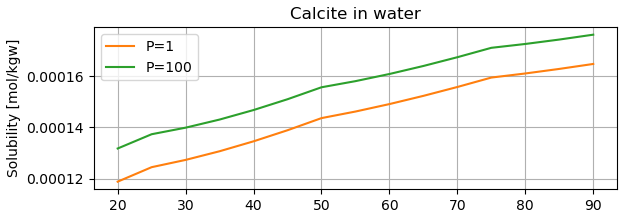
\includegraphics[height=2.2cm]{figures/chemical-equilibrium/calcite-solubility-water.png} \quad
	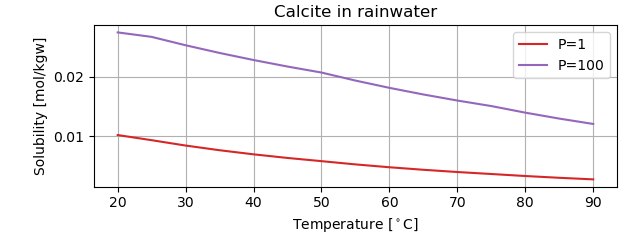
\includegraphics[height=2.2cm]{figures/chemical-equilibrium/calcite-solubility-rainwater.png}
	\caption*{\footnotesize Calcite solubility in water and rain water w.r.t. temperature.}
\end{figure}
\end{frame}

%
% --------------------------------------------------------------------------------------------------------------------%
% Calcite solubility example -- Stalagmites and stalactites
% --------------------------------------------------------------------------------------------------------------------%
%
\begin{frame}{Calcite solubility example,  Stalagmites and stalactites}

\[\mathsf{CaCO_3(s) + CO_2(g) + H_2O(l) \rightleftharpoons Ca(HCO_3)_2(aq)}\]

\vskip -10pt
\begin{columns}[t]
\column{0.3\textwidth}
\vskip 10pt
$\rightarrow$ Rainwater meets with limestone to form a solution of calcium bicarbonate. \\[5pt]
$\leftarrow$ The bicarbonate-rich water drips from the ceiling of the cave and partially evaporates, leaving behind a calcium carbonate deposit.

\column{0.7\textwidth}

\begin{figure}\centering
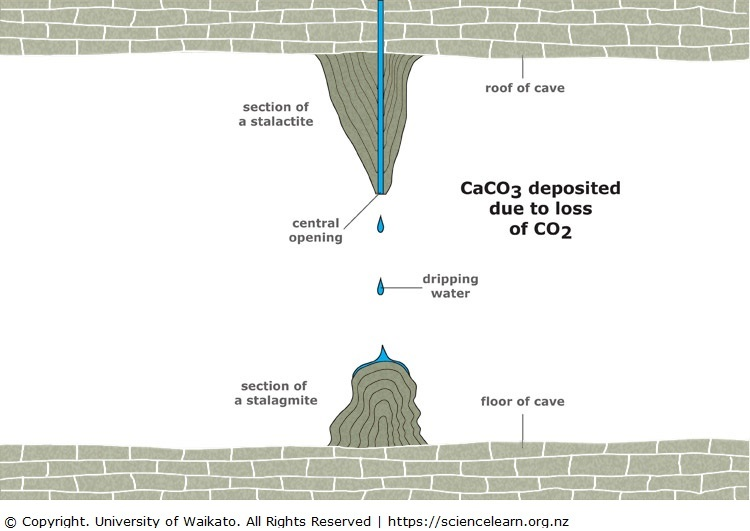
\includegraphics[width=0.7\textwidth]{figures/chemical-equilibrium/stalagmites-stalactities.jpg}
\caption{\footnotesize
Diagram of cave showing formation of stalagmites and stalactites.}
\end{figure}

\end{columns}

\end{frame}
%
% --------------------------------------------------------------------------------------------------------------------%
% Calcite solubility example -- Limestone fizzing
% --------------------------------------------------------------------------------------------------------------------%
%
\begin{frame}{Calcite solubility example,  Limestone fizzing}

\vskip 10pt
\begin{figure}
\centering
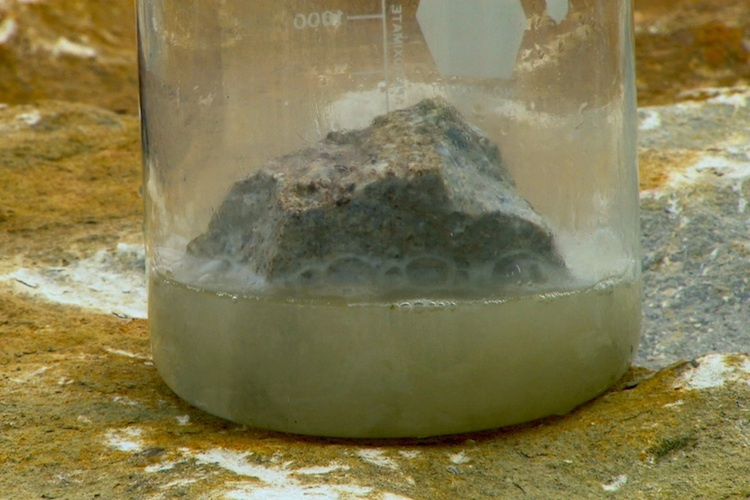
\includegraphics[width=0.65\textwidth]{figures/chemical-equilibrium/limestone-fizzing.jpg}
\caption{Limestone fizzes when dilute acid is placed on its surface.}
% When dilute acid is placed on a sample of limestone rock, it fizzes. 
% The calcium carbonate present in the limestone is reacting with the acid to produce carbon dioxide gas.
\end{figure}

\end{frame}
%
% --------------------------------------------------------------------------------------------------------------------%
% Solubility of chlorargyrite, Example
% --------------------------------------------------------------------------------------------------------------------%
%
\begin{frame}{Solubility of chlorargyrite, Example}
	%
	\begin{itemize}
		\item Consider dissolution reaction of chlorargyrite 
		\[
		\mathsf{AgCl(s) \rightleftharpoons Ag^{+}(aq) + Cl^{-}(aq)}
		\]
		%
		\item  \alert{\bf Quiz}: What is solubility of AgCl(s) in 1 liter of water, where $K_{sp} = 1.8 \cdot 10^{-10}$?
		\begin{center}
			\href{http://etc.ch/oyhr}{\textcolor{indigo(dye)}{\tt http://etc.ch/oyhr}} 
			\quad
			or 
			\quad
			
\includegraphics[height=0.2\columnwidth]{figures/chemical-equilibrium/poll-mass-balance.png}
		\end{center}
		\hiddenpause
		\item {\bf Answer}: 1 liter of water can dissolve $1.34 \cdot 10^{-5}$ mol/L of AgCl(s) at room temperature. \\
		%
		{\bf Note}: Compared with other types of salts, AgCl is also poorly soluble in water. \\
		In contrast, table salt NaCl has a higher $K_{sp}$ and is, therefore, more soluble.
	\end{itemize}
\end{frame}		
%
% --------------------------------------------------------------------------------------------------------------------%
% Saturation index
% --------------------------------------------------------------------------------------------------------------------%
%
\begin{frame}{Saturation index}

The \alert{\textbf{saturation index}} indicates the saturation state of
a solution with respect to a mineral phase, which is given by
%
\[
\boxed{ \mathrm{SI} = \log_{10} \frac{Q}{K_{sp}}},
\] 
where 
\begin{itemize}
\item $Q$ is the \emph{ion activation product (IAP) / reaction quotient} of activities of the dissolved species (characteristic of non-equilibrium solution), 
and 
\item $K_{sp}$ is the \emph{solubility product / equilibrium constant}. 
\end{itemize}
%
\[
\mathrm{SI} \quad \begin{cases}
< 0& \mbox{solution is \textbf{undersaturated} $\Rightarrow$ the mineral may be dissolved }\\
= 0& \mbox{solution is \textbf{saturated} \qquad \; $\Rightarrow$ the mineral in equilibrium with solution}\\
> 0 & \mbox{solution is \textbf{supersaturated} $\Rightarrow$ the mineral may be precipitated}
\end{cases}
\]
%
%The solubility of a given solute can be determined with the solubility product.

\end{frame}
%
% --------------------------------------------------------------------------------------------------------------------%
% Saturation index, Example
% --------------------------------------------------------------------------------------------------------------------%
%
\begin{frame}{Saturation index, Exercise}
	
%	BaSO4(s)↽−−⇀Ba2+(aq)+SO2−4(aq)
%	Barium sulfate is used in medical imaging of the gastrointestinal tract. Solubility product of barium sulfate is 1.08×1e-10 at 25°C
%	
%	Will barium sulfate precipitate if 10.0 mL of 0.0020 M Na2SO4 is added to 100 mL of 3.2 × 10−4 M BaCl2? 
%	[Ba2+]=2.9×10−4 molal
%	[SO2−4]=1.8×10−4 molal
%	IAP = 5.2×10−8
%	IAP > Ksp: we predict that BaSO4BaSO4 will precipitate when the two solutions are mixed. In fact, BaSO4BaSO4 will continue to precipitate until the system reaches equilibrium, which occurs when 1.08×1e-10 is reached.

	\begin{itemize}
		\item Consider dissolution reaction of barium sulfate 
		\[
		\mathsf{BaSO_4(s) \rightleftharpoons Ba^{2+}(aq) + SO_4^{2-}(aq).}
		\]
		%
		\item Solubility product of barium sulfate is 1.08e-10 at 25 ${\rm ^\circ}$C.
		%
		\item  \alert{\bf Quiz}: What can be said about the water w.r.t. to barium sulfate if \\
		${\sf [Ba^{2+}}]=2.9 \cdot$ 1e-4 molal
		${\sf [SO_4^{2-}]}=1.8 \cdot$ 1e-4 molal?
		%
		\begin{center}
			\href{http://etc.ch/oyhr}{\textcolor{indigo(dye)}{\tt http://etc.ch/oyhr}} 
			\quad
			or 
			\quad
			
\includegraphics[height=0.2\columnwidth]{figures/chemical-equilibrium/poll-mass-balance.png}
		\end{center}
		\hiddenpause
		\item {\bf Answer}: Water will be supersaturated with ${\sf BaSO_4(s)}$.
	\end{itemize}

\end{frame}
%
% --------------------------------------------------------------------------------------------------------------------%
% Saturation index, Demonstration
% --------------------------------------------------------------------------------------------------------------------%
%
\begin{frame}{Saturation index, Demonstration}
	
	\lcol
	\vskip -5pt
	\begin{itemize}
		\item Demonstration of gypsum/anhydrite solubility: 
		%
		Jupyter notebook tutorial 
		\href{https://github.com/mtsveta/reaktoro-jupyter/blob/geofluids-examples/tutorial/eq.anhydrite-solubility.ipynb}{\textcolor{indigo(dye)}{\it Gypsum/anhydrite solubility in water}}.
		%
		\item Investigation on how saturated the Evian water with carbonates can be found in 
		Jupyter notebook tutorial \href{https://github.com/mtsveta/reaktoro-jupyter/blob/geofluids-examples/tutorial/eq.evian-water-analysis.ipynb}{\textcolor{indigo(dye)}{\it Analysis of the Evian water}}.
		%
		\item Barite precipitation in the water flooding reactive transport example:
		%
		Jupyter notebook tutorial 
		\href{https://github.com/mtsveta/reaktoro-jupyter/blob/master/tutorial/rt.scaling.ipynb}{\textcolor{indigo(dye)}{\it One-dimensional reactive transport modeling of scaling (without oil)}}.
		
	\end{itemize}
	%
	\rcol
	\begin{figure}
		\centering
		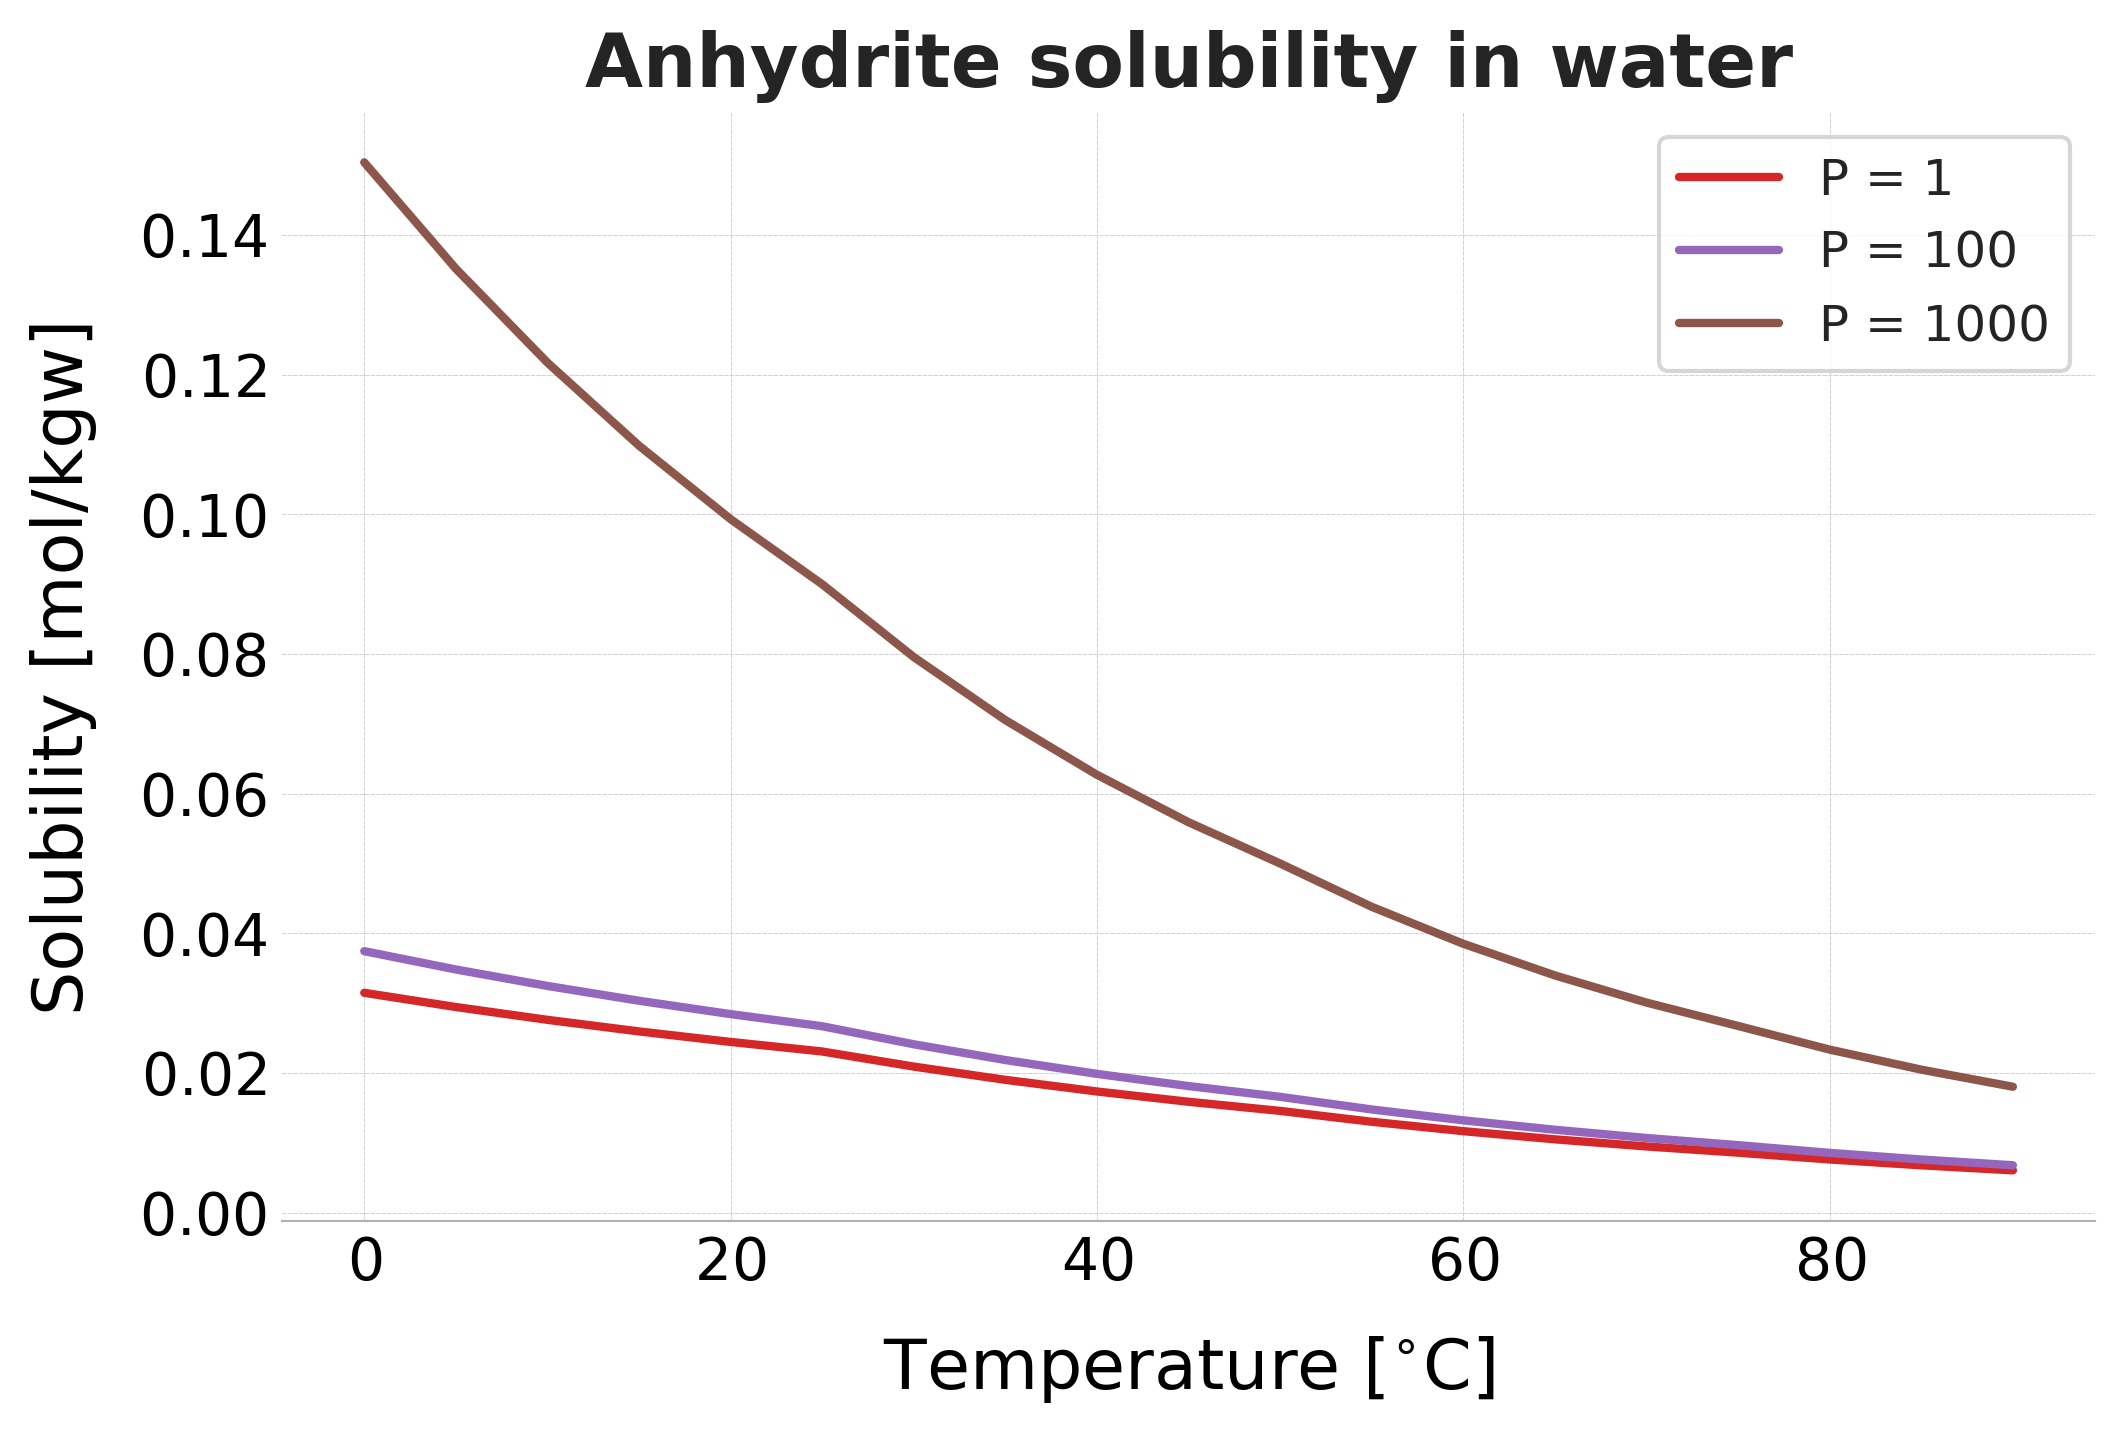
\includegraphics[width=0.8\columnwidth]{figures/chemical-equilibrium/anhydrite-solubility.png}
		%\caption{}
	\end{figure}
	\vskip -10pt
	\begin{figure}
		\centering
		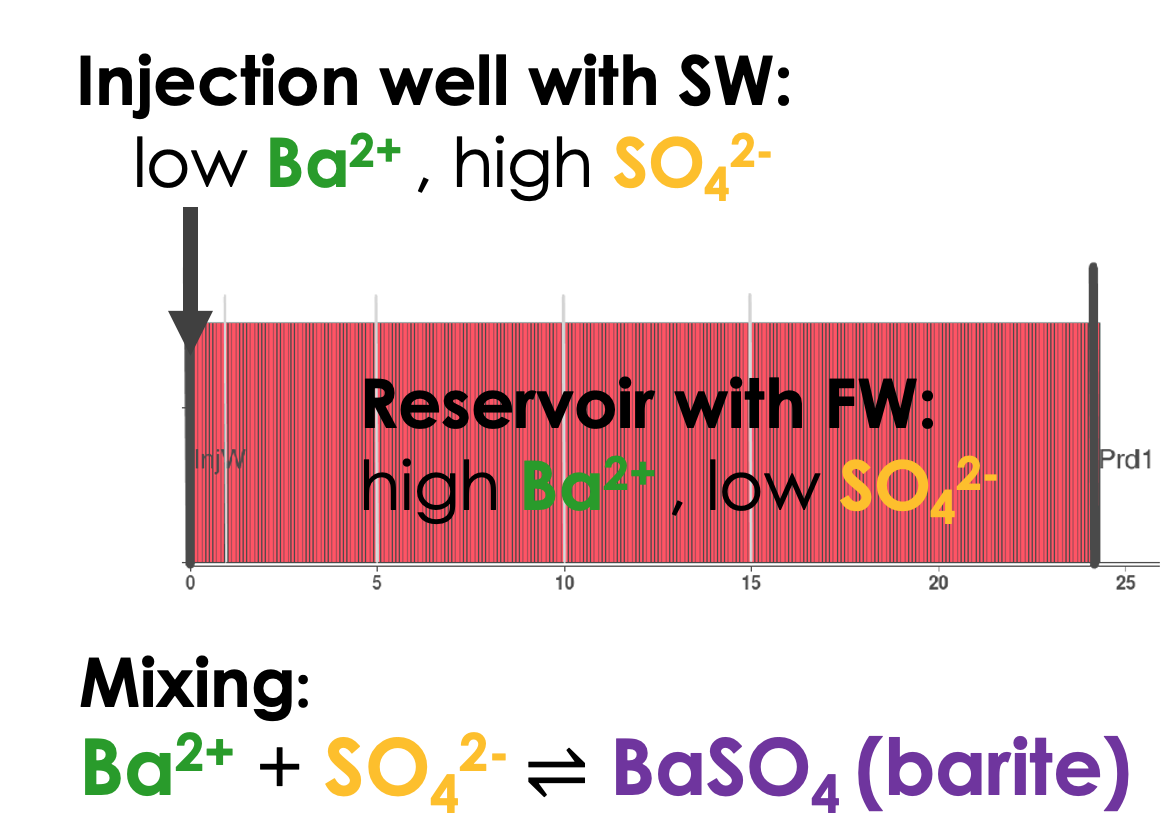
\includegraphics[width=0.75\columnwidth]{figures/chemical-equilibrium/barite-scaling.png}
		%\caption{}
	\end{figure}
	\ecol
	
	%\begin{itemize}
	%\item Demonstration of gypsum solubility: 
	%%
	%Jupyter notebook tutorial 
	%\href{}{\textcolor{indigo(dye)}{\it }}.
	%%
	%%
	%\item Barite precipitation in the water flooding RT example 
	%%
	%Jupyter notebook tutorial 
	%\href{}{\textcolor{indigo(dye)}{\it Calcite solubility in water and CO$_2$-saturated rainwater}}.
	%\end{itemize}
\end{frame}
	
%\begin{frame}{Barite scaling model illustration}
%	\centering
%	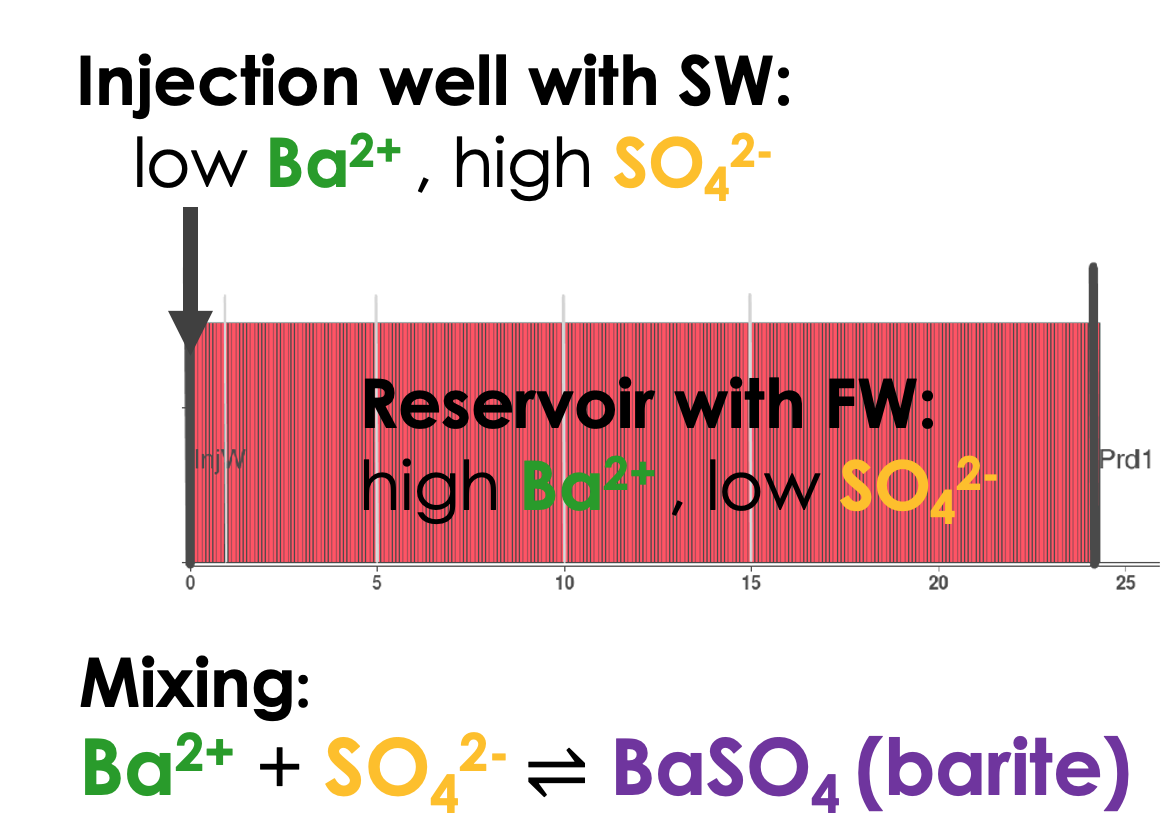
\includegraphics[width=0.75\columnwidth]{figures/chemical-equilibrium/barite-scaling.png}
%\end{frame}

%
%
% --------------------------------------------------------------------------------------------------------------------%
% Electroneutrality principle
% --------------------------------------------------------------------------------------------------------------------%
%
\begin{frame}{Electroneutrality principle}

\begin{itemize}
\item \alert{\textbf{Electroneutrality principle}} (Pauling, 1948) states that 
the ionic species in the electrolyte solution have equilibrium of charges on a macroscopic scale.
\pause
\item It can be expressed by the charge equilibrium between the species in solution
%
\[
\boxed {\sum_i Z_i m_i = 0,}
\]
%
where $Z_i$ are the ionic charges and 
$m_i$ are the molalities of species.
%
\pause 
\item \alert{\bf Example}: 
When mixing 0.1 molal of NaCl, it dissolves to 0.1 molal Na$^+$ and 0.1 molal Cl$^-$.

\end{itemize}
%
\end{frame}
%
% --------------------------------------------------------------------------------------------------------------------%
% Reduction/oxidation potential, pE
% --------------------------------------------------------------------------------------------------------------------%
%
\begin{frame}{Reduction/oxidation potential, pE}
\begin{itemize}
	\item  \alert{\textbf{Oxidation / reduction}} are the reactions, where species either esquire or lose electors, e.g., 
	%
	%\item Species in an aqueous solution can {\bf donate or accept electrons}, for example:
	%
	\[
	\mathsf{e^- + \tfrac{1}{4} \, O_2(aq) + H^+ = \tfrac{1}{2} \, H_2O.}
	\]
	\vskip -10pt
	%
	\pause
\item \alert{\textbf{Oxidation / reduction potential}} is a {\bf measure of the tendency} of a species to acquire/lose electrons from/to an electrode and thereby {\bf be reduced or oxidised}. 
%But such reaction is rather used as a {\bf half-reaction}. Additional half-reaction must be written to result into {\bf a charge-balanced equation}.
%. 
%
	\pause
\item The \alert{\textbf{reduction/oxidation potential}} $\mathsf{pE}$ is defined as
%
\[
\boxed{ \mathsf{pE} = - \log_{10} (a_{e^{\scalebox{0.75}[1.0]{-}}}) = -\tfrac{1}{n_e} \log \tfrac{Q^{\scalebox{0.75}[1.0]{-}}_e}{K^{\scalebox{0.75}[1.0]{-}}_e} }
\]
\vskip -5pt
%
where 
\begin{itemize}
	\item $K^{\scalebox{0.75}[1.0]{-}}_e \approx 25.5$ (at 25 \textdegree C), 
	\item $n_e$ is the number of consumed/generated electrons, and 
	\item $Q^{\scalebox{0.75}[1.0]{-}}_e$ is the product of the activities of the reaction. 
\end{itemize}
%
	\pause
\item A solution with a {\bf higher pE} /  {\bf lower pE} will have a tendency to {\bf gain electrons from} / {\bf lose electrons to} the new species.
%
\end{itemize}

\end{frame}
%
% --------------------------------------------------------------------------------------------------------------------%
% Hydrogen potential, pH
% --------------------------------------------------------------------------------------------------------------------%
%
\begin{frame}{Hydrogen potential, pH}

\begin{itemize}
	\item The \alert{\textbf{$\mathsf{pH}$}} of a solution is an indication of the \textbf{tendency} of the solution \textbf{to donate hydrogen ions}
	or measure of the \textbf{relative amount of free hydrogen ions} in the solution. 
	%
		\pause
	
\item The \alert{\textbf{hydrogen potential}} $\mathsf{pH}$ is defined as
%
\[
\boxed{ 
\mathsf{pH} = - \log_{10} (a_{\mathsf{H^+}}) = - \log_{10} ([H^+]). 
}
\]
%
\vskip -10pt
	\pause
\item $\mathsf{pH}$ is a measure of how \textbf{acidic/basic} solution is in the scale from 0 till 14: 
%
%\begin{alignat*}{2}
%\mathsf{pH} < 7: & \qquad \mbox{solution is \textbf{acidic}}\\
%\mathsf{pH} = 7: & \qquad \mbox{solution is \textbf{neutral}}\\
%\mathsf{pH} > 7: & \qquad  \mbox{solution is \textbf{alkali/base}}
%\end{alignat*}
%
%\[
%\mathsf{pH} < 7: \; \mbox{solution is \textbf{acidic}} \qquad
%\mathsf{pH} = 7: \; \mbox{solution is \textbf{neutral}} \qquad
%\mathsf{pH} > 7: \; \mbox{solution is \textbf{alkali/base}}
%\]
\end{itemize}
\begin{figure}
\centering
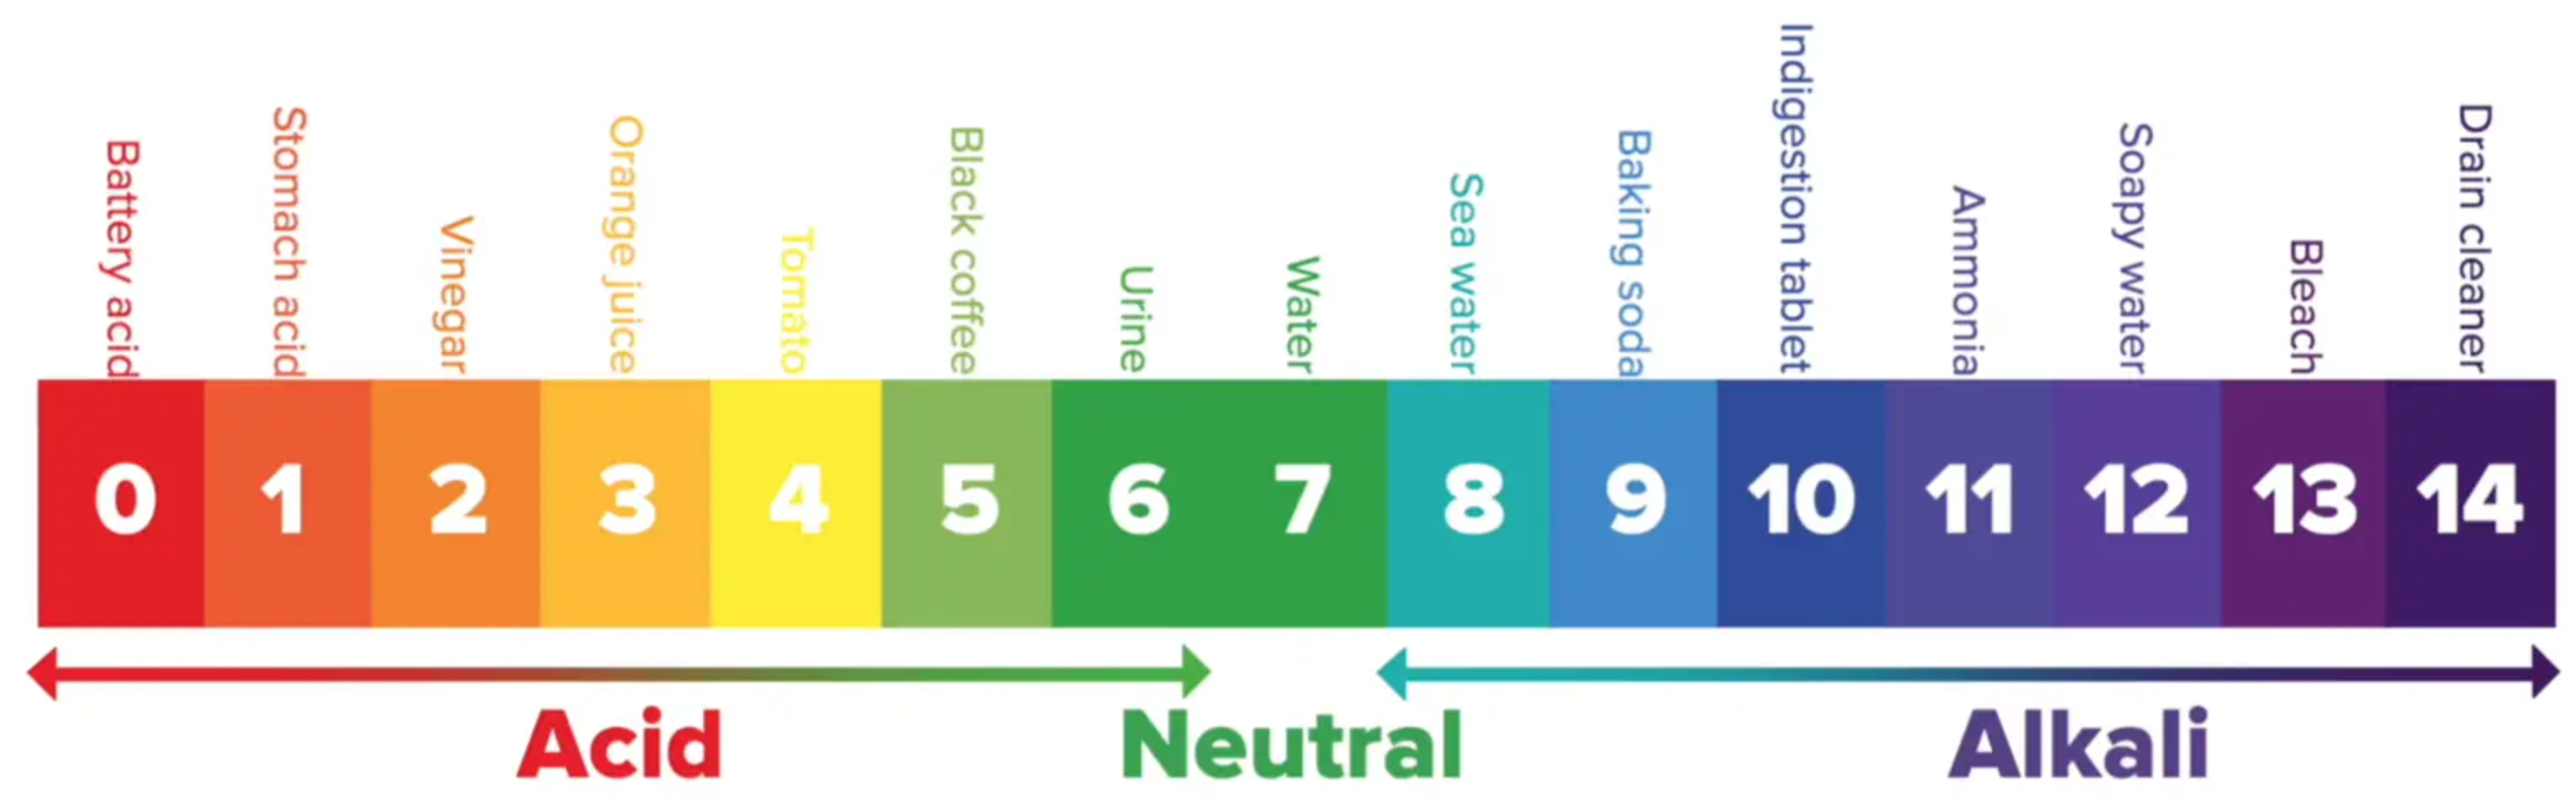
\includegraphics[width=0.9\columnwidth]{figures/chemical-equilibrium/ph-scale.png}
\end{figure}
\end{frame}
%
% --------------------------------------------------------------------------------------------------------------------%
% Saturation index, Example
% --------------------------------------------------------------------------------------------------------------------%
%
\begin{frame}{pH, Exercise}
	\small
	\begin{itemize}
		\item We have completely dissolved HCl in the 300 ml of water  
		%
		$\mathsf{HCl(aq) \rightleftharpoons H^+(aq) + Cl^-(aq)}$
		%
		%
		 and it produced the solution with pH = 1. 
		%
		\pause
		\item {\bf Hint 1}: let the concentration $[\mathsf{H^+}]$ (measured in mol/L) and $a_{\mathsf{H^+}}$ be the same (i.e., activity is considered as effective concentration). 
		%
		\item {\bf Hint 2}: $m_{\mathsf{HCl}} = M_{\mathsf{HCl}}  \cdot n_{\mathsf{HCl}},$ 
		%
		where $m$ is the mass of species (in kg), 
		$M$ is the molar mass (in kg / mol), and 
		$n$ is the molar amount (in mol). 
		%
		\item {\bf Hint 3}: molar amount of $M_{\mathsf{HCl}} = $ 36.458 g/mol .
		%
		\pause
		\item  \alert{\bf Quiz}: What was the mass of dissolved HCl?
		%
		\begin{center}
			\href{http://etc.ch/oyhr}{\textcolor{indigo(dye)}{\tt http://etc.ch/oyhr}} 
			\quad
			or 
			\quad
			
\includegraphics[height=0.2\columnwidth]{figures/chemical-equilibrium/poll-mass-balance.png}
		\end{center}
		\hiddenpause
		\item {\bf Answer}: 1.09374 g. 
	\end{itemize}
	
\end{frame}
% --------------------------------------------------------------------------------------------------------------------%
% pH, Examples i
% --------------------------------------------------------------------------------------------------------------------%
%
\begin{frame}{pH, Examples \; i}
	
	\lcol
	\vskip -5pt
	\begin{itemize}
		\item Too high or too low pH effect aquatic / fish life. 
		\pause
		\item 
	Large \alert{\textbf{algae blooms}} can affect the pH as they photosynthesise: 
	\begin{itemize}
		\item during the day that \textbf{drives the pH down} and 
		\item at night when they respire, it \textbf{drives the pH up}.
		%
	\end{itemize}
	%
	\alert{\textbf{The results}}: \textbf{huge pH fluctuations} in water, which can affect fish quite negatively. 
	\end{itemize}
	%
	\rcol
	%\vskip -30pt
	\begin{figure}
		\centering
		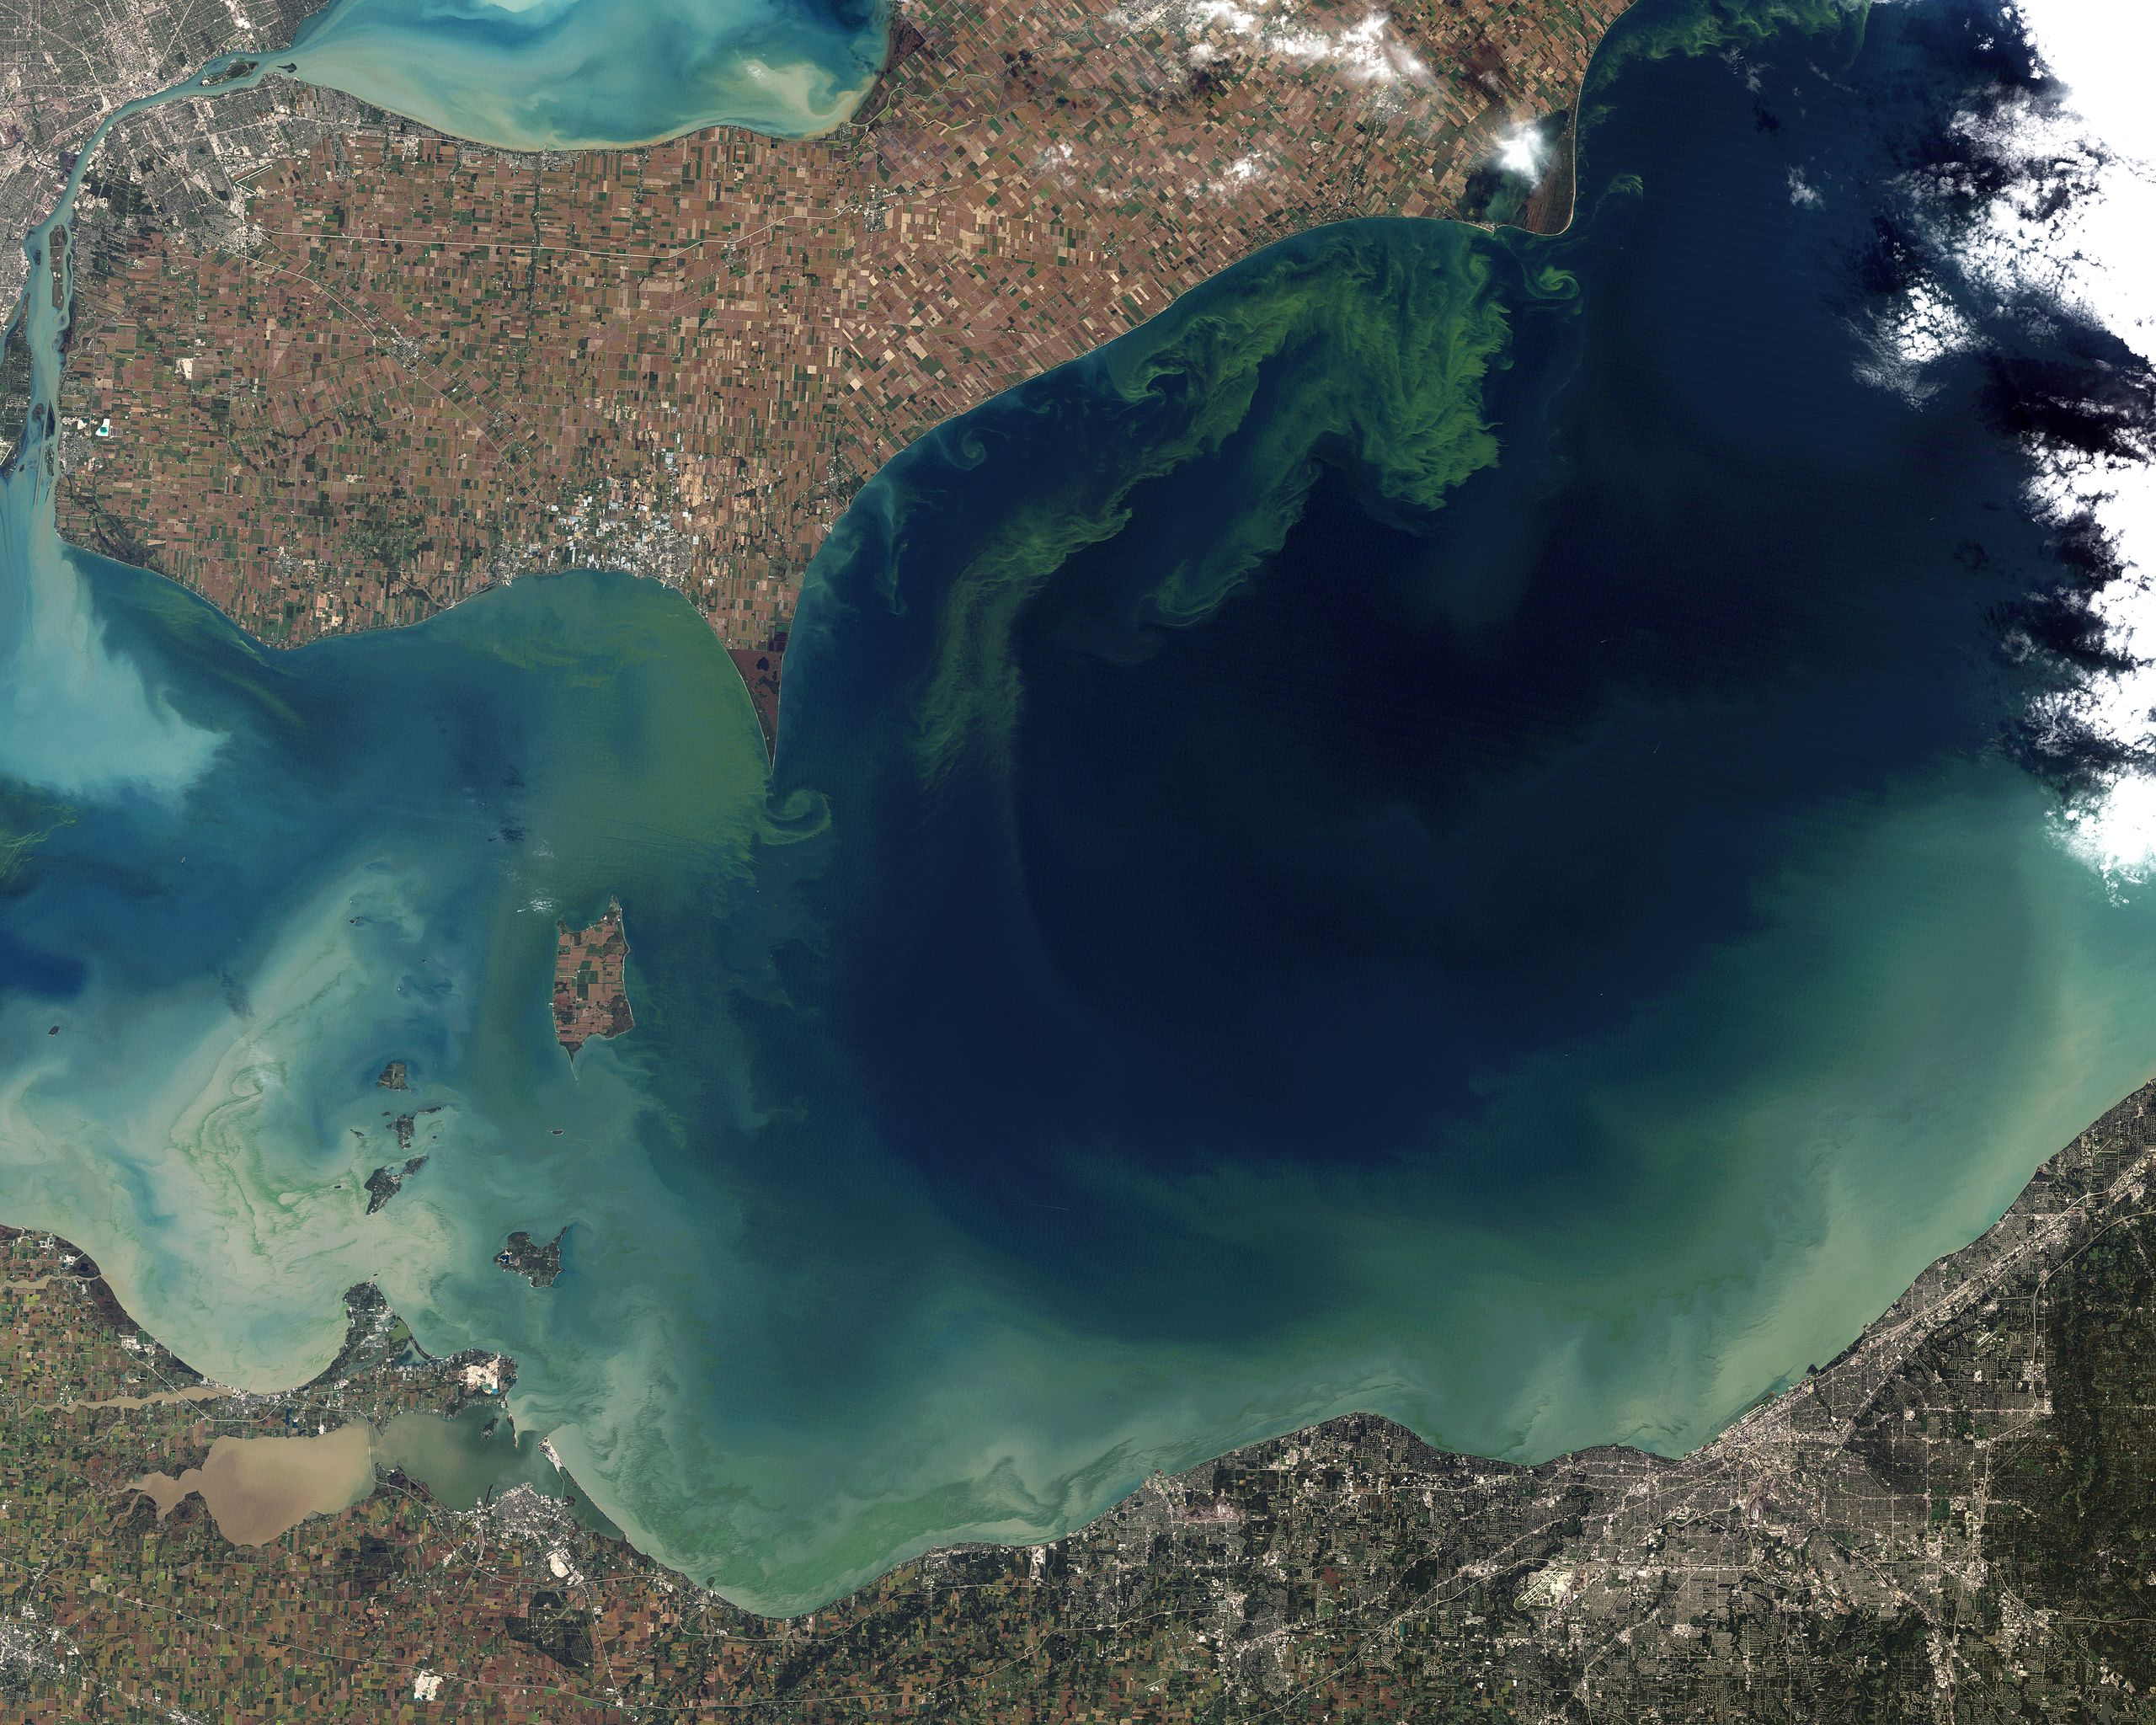
\includegraphics[width=0.85\columnwidth]{figures/chemical-equilibrium/toxic_algae_bloom_lake_erie.jpg}
		\caption{\small The worst algae bloom that Lake Erie has experienced in decades resulting from the record torrential spring rains washed fertilizer into the lake, promoting the growth of microcystin-producing cyanobacteria blooms.}
	\end{figure}

	\ecol
	
\end{frame}
%
% --------------------------------------------------------------------------------------------------------------------%
% pH, Examples ii
% --------------------------------------------------------------------------------------------------------------------%
%
\begin{frame}{pH, Examples \; ii}
\footnotesize
\lcol

\begin{itemize}
\item $\mathsf{CO_2}$ added to the seawater influences the $\mathsf{pH}$ according to the reaction
%
\[
\mathsf{CO_2(g) + H_2O(l) = H^+ + HCO_3^-.}
\]
% 
See tutorial \href{}{\textcolor{indigo(dye)}{\it Dependence of the pH on the $\mathsf{CO_2(g)}$ amount in seawater}}.
%
\pause
\vskip 10pt
\pause
\item Adding HCl into water increases free $\mathsf{H^+}$ ions and decreases pH according to the reaction 
%
\[
\mathsf{HCl(aq) + H_2O(l) = H_3O^+ + Cl^-,}
\]
%
whereas 
%Water and HCl combine to form \textbf{hydrochloric acid} ($\mathsf{H_3O^+}$ and $\mathsf{Cl^-}$):
%
%\[
%\mathsf{HCl(aq) + H_2O(l) = H_3O^+ + Cl^-.}
%\]
%
adding ammonia \textbf{removes} $\mathsf{H^+}$ from water and increases it to produce ammonium and hydroxide, i.e., 
%to produce ammonium and hydroxide:
%
\[
\mathsf{NH_3 + H_2O = NH_4^+ + OH^-.}
\]
%
%
%By adding acid, we decrease the $\mathsf{pH}$ of water
%%
%\[
%\mathsf{HCl(aq) + H_2O(l) = 2\, H^+ + HO^- + Cl^-.}
%\]
% 
See tutorial \href{}{\textcolor{indigo(dye)}{\it Dependence of the pH on added contaminant in water}}.

\end{itemize}
%
\rcol
\begin{figure}
\centering
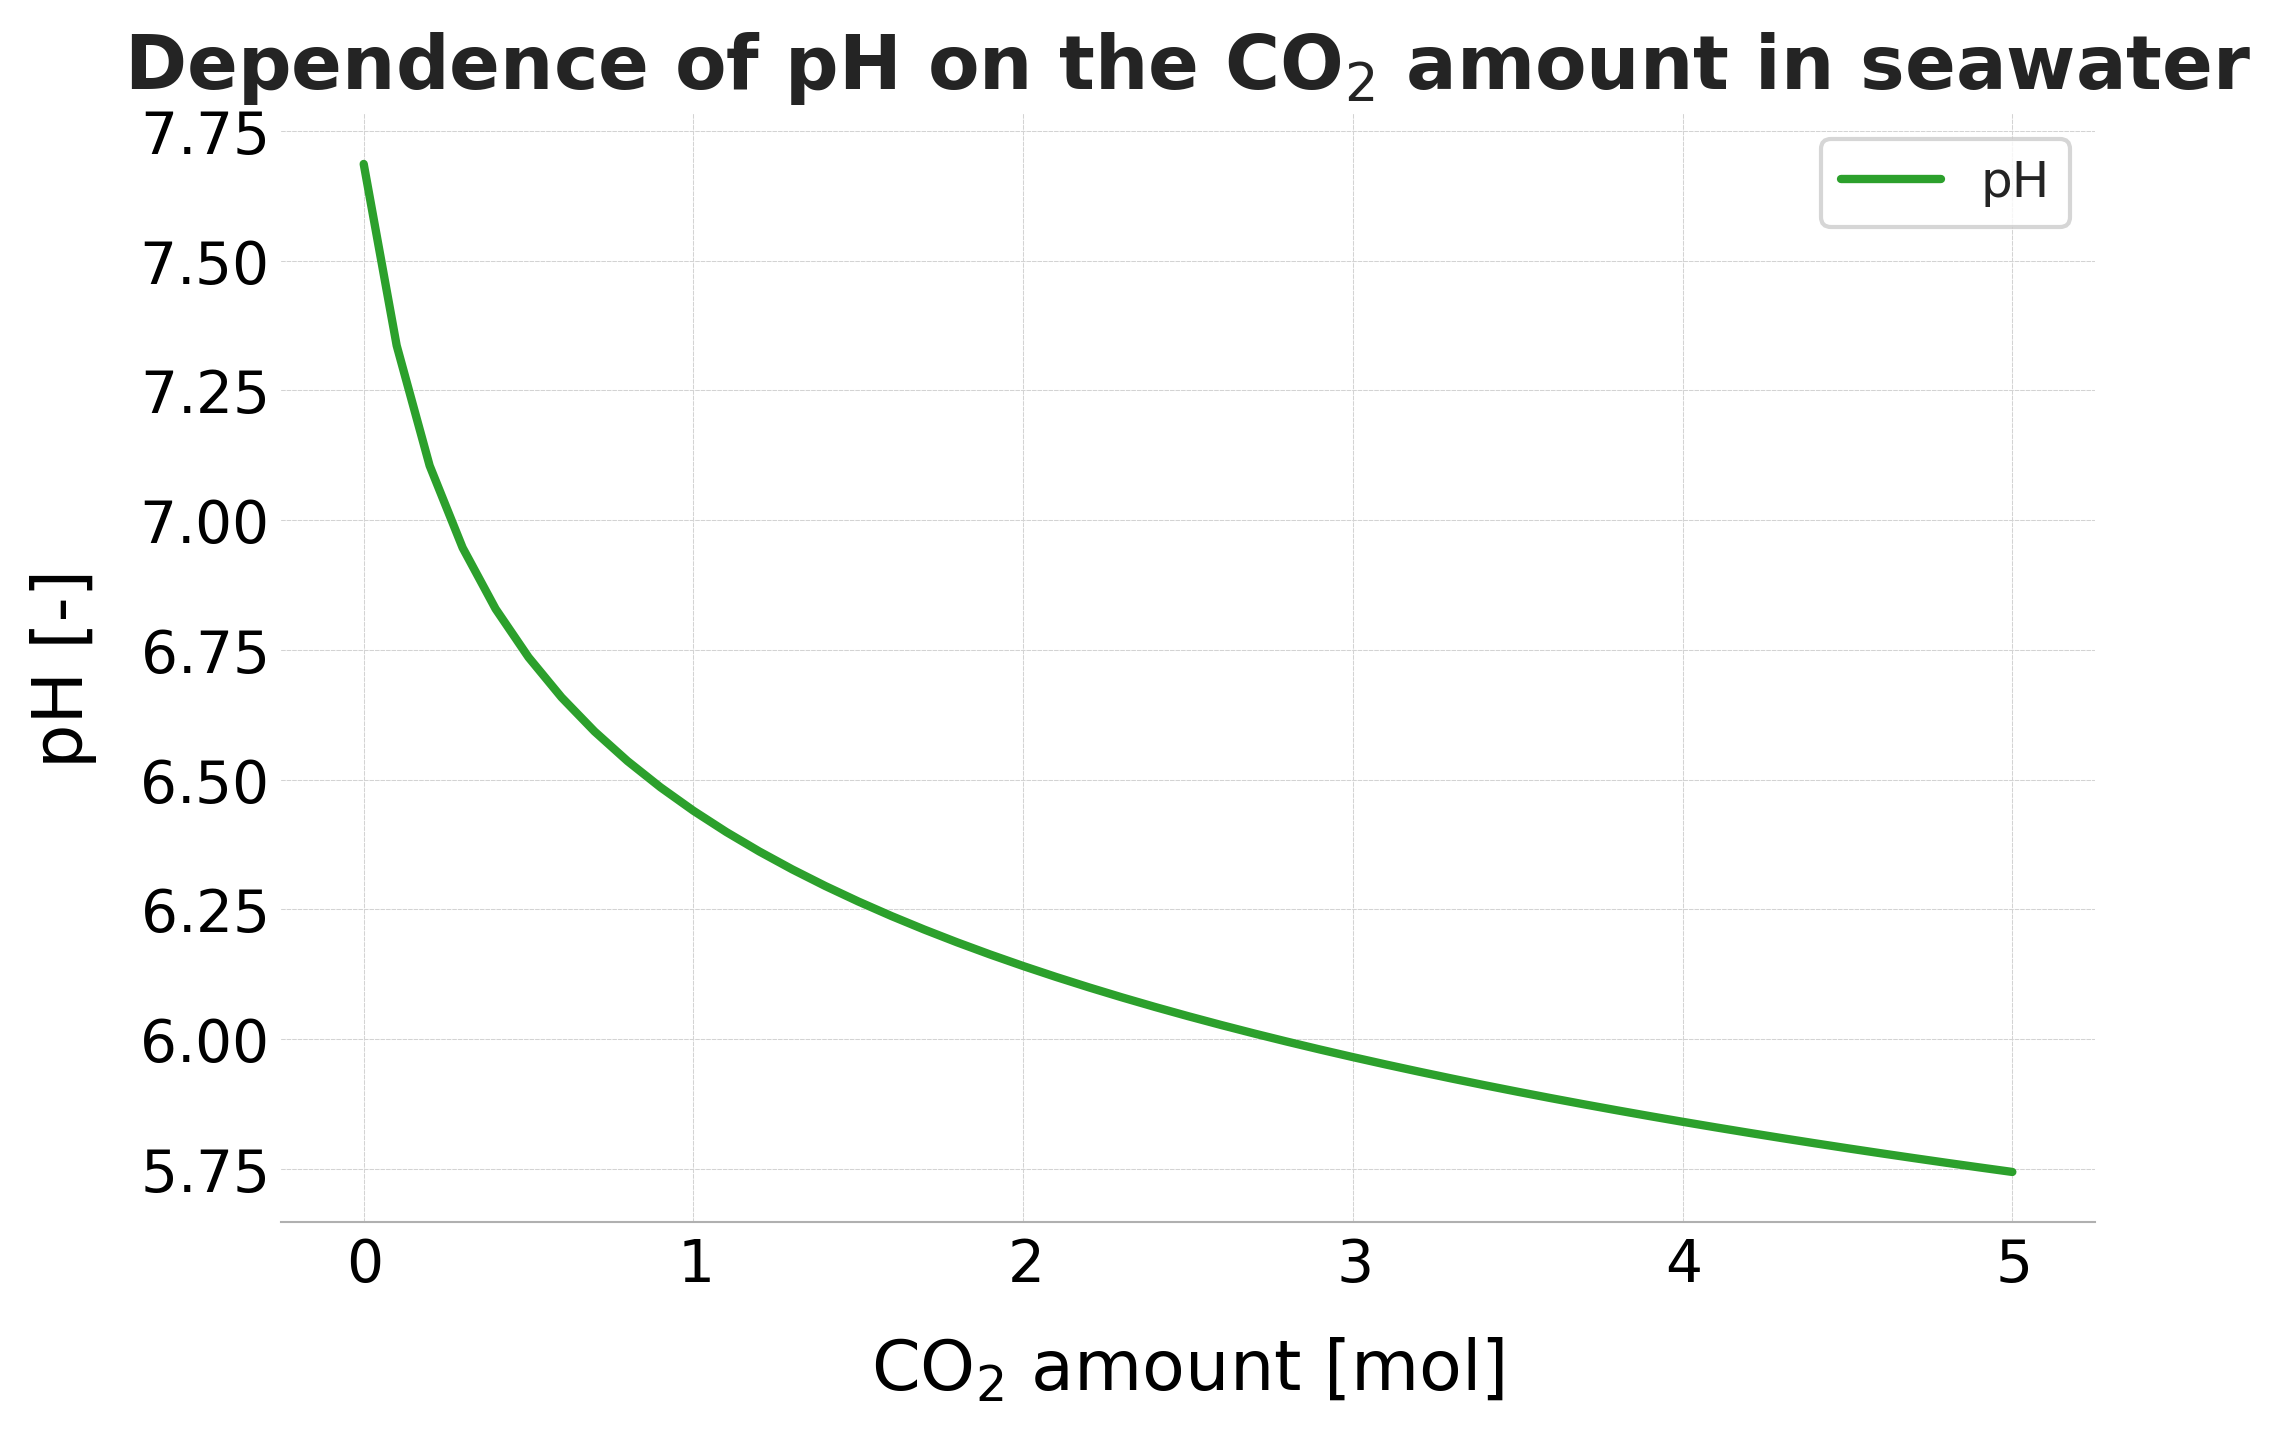
\includegraphics[width=0.82\columnwidth]{figures/chemical-equilibrium/ph-dependence-on-co2-amount-in-seawater.png}
%\caption{}
\end{figure}
\vskip -10pt
\begin{figure}
\centering
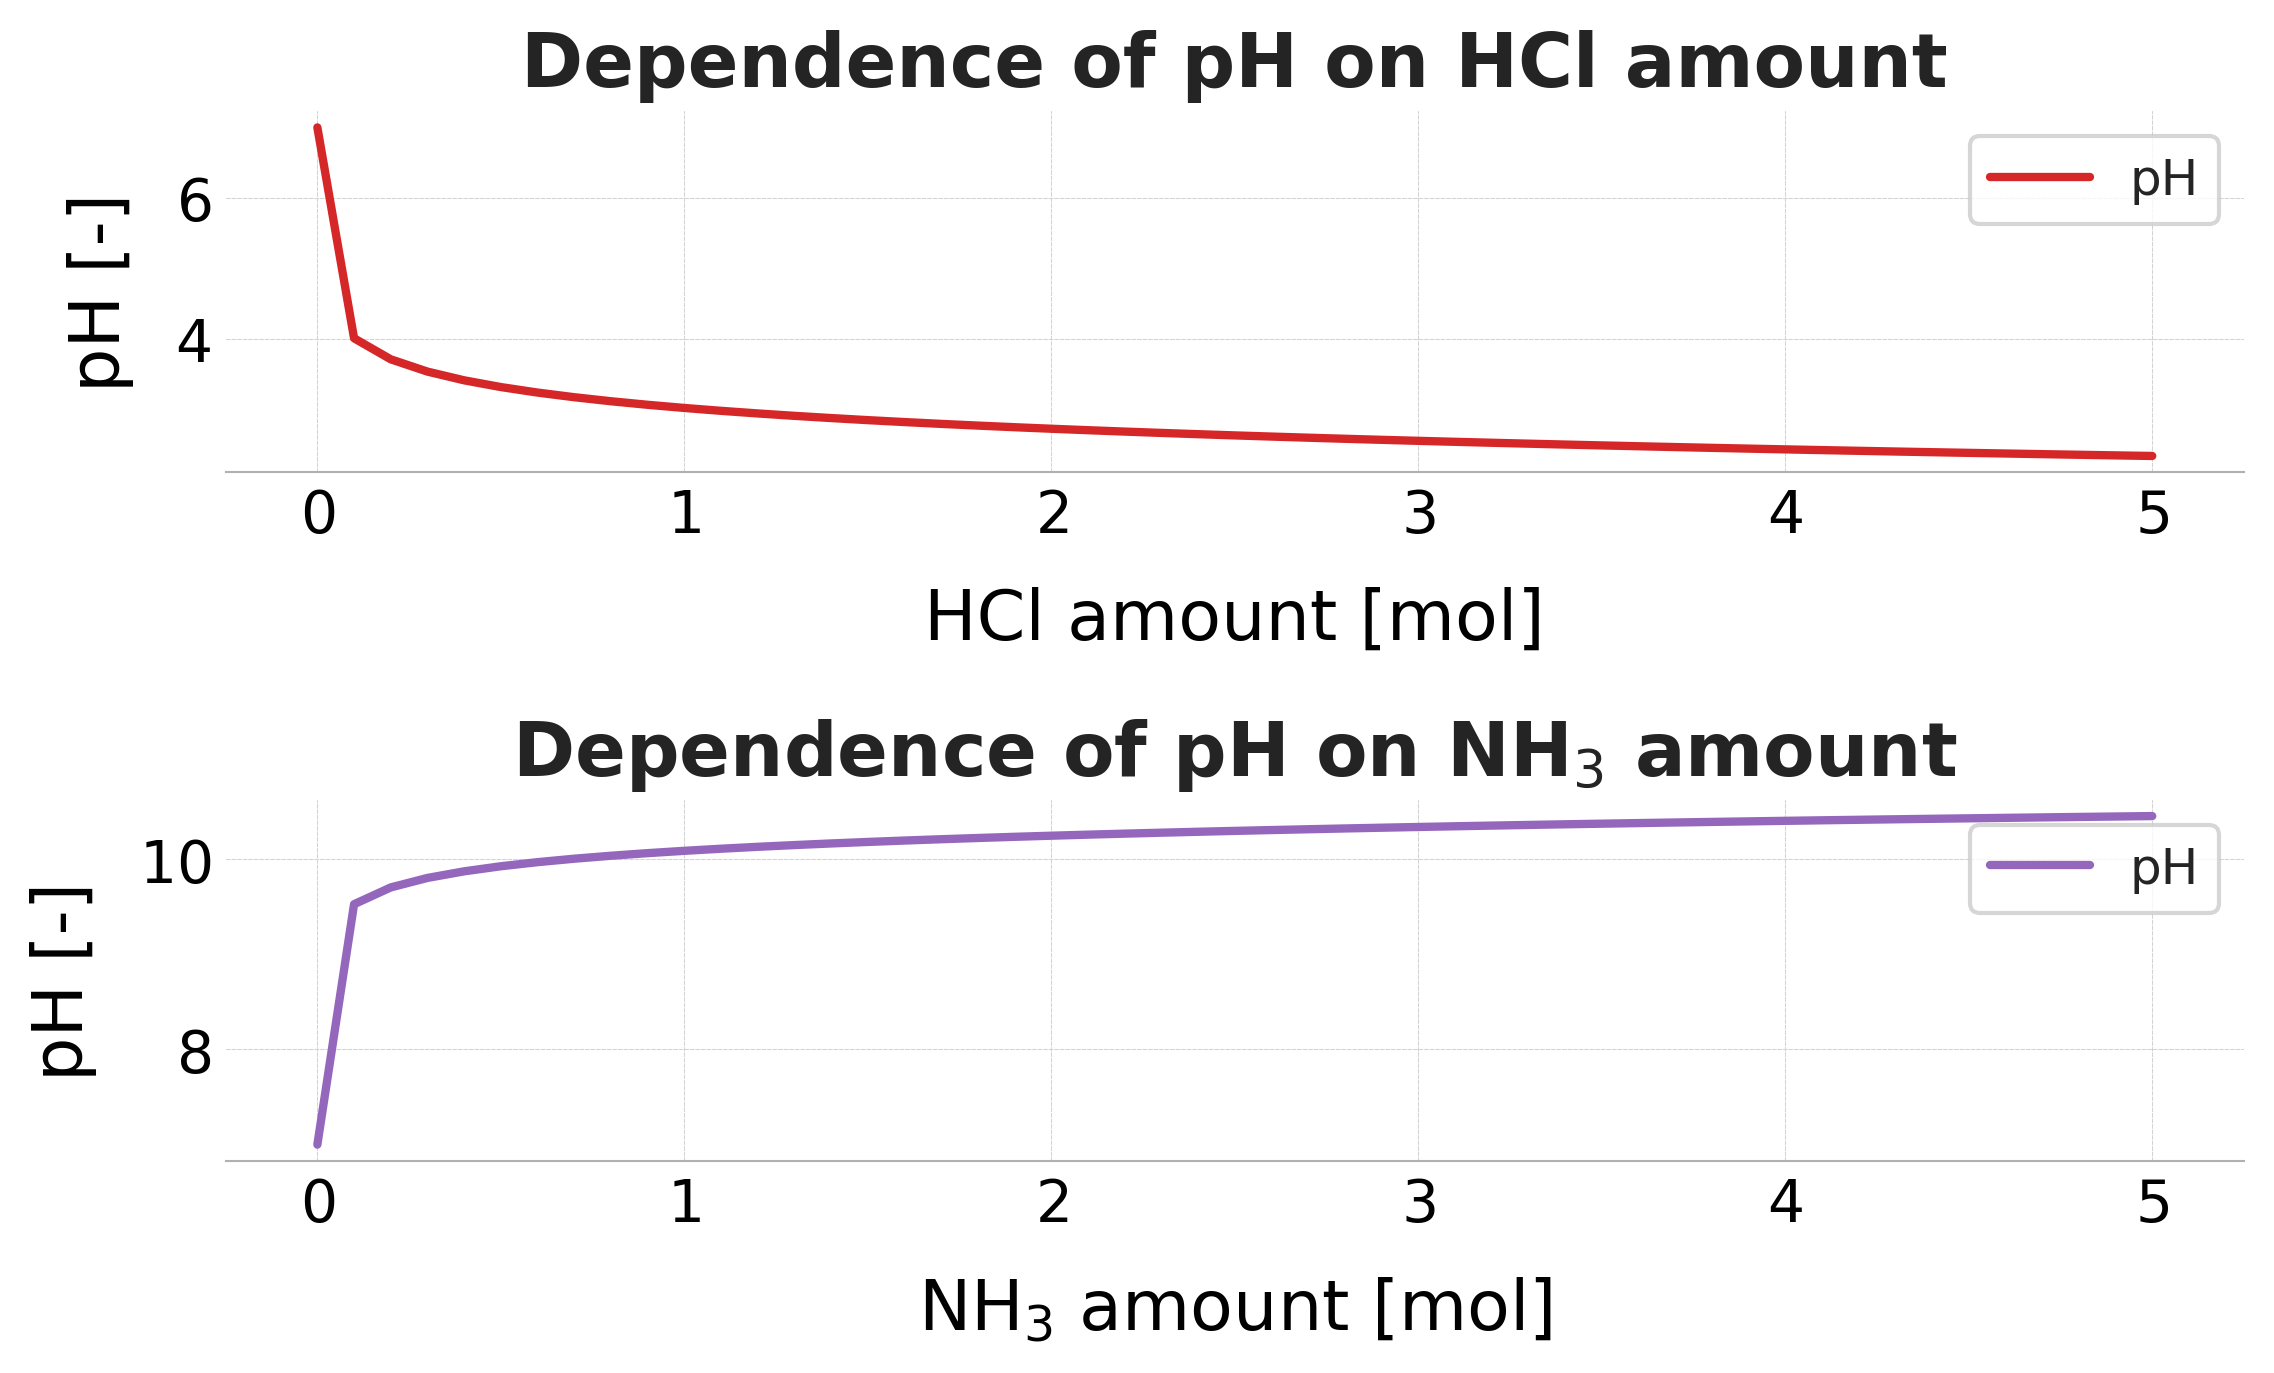
\includegraphics[width=0.82\columnwidth]{figures/chemical-equilibrium/ph-dependence-on-contaminants-in-water.png}
%\caption{}
\end{figure}
\ecol

\end{frame}



